\documentclass[pfe ,titlesmallcaps]{isipfe}
\usepackage[T1]{fontenc}
\usepackage[utf8]{inputenc}
\graphicspath{{./Figures/}}
\usepackage{hyperref}
\usepackage{algorithm}
\usepackage{algorithmic}
\usepackage{float}
\usepackage{acronym}
\usepackage{textcomp}
\usepackage[british,UKenglish,USenglish]{babel}
\usepackage{enumitem}
\usepackage{multirow}
\usepackage{graphicx}
\usepackage{array}
\usepackage{booktabs}
\usepackage{ltxtable}
\usepackage[table]{xcolor}
\usepackage{colortbl}
\usepackage{arabtex}
\usepackage{pdfpages}
\usepackage{utf8}
\usepackage{tcolorbox}
%fixing space in list of figures
\usepackage[titles]{tocloft}
\cftsetindents{figure}{0em}{3em}
\cftsetindents{table}{0em}{3em}


\usepackage{titleps}% http://ctan.org/pkg/titleps

\newcounter{para}
\newcommand\mypara[1]{\par\refstepcounter{para}\textbf{\thepara\space}}
\begin{document}  

\frontmatter

\title{Titre du projet}
\author{Prénom NOM}

%%% YOU MUST update information of this page
\thispagestyle{empty}
\hspace{-1cm}
\begin{minipage}[l]{0.2\columnwidth}

\includegraphics[width=1.1\columnwidth]{LogoISI}\\
\end{minipage}
\hfill
\begin{minipage}[l]{0.6\columnwidth}
\centering
\footnotesize

\textbf{\textsc{Ministry of Higher Education\\
and scientific research}}\\
\textbf{\textsc{University of Tunis Al Manar}}\\
\textbf{\textsc{higher institute of computer science}}
\end{minipage}
\hfill
\begin{minipage}[l]{0.2\columnwidth}

\includegraphics[width=0.7\columnwidth]{logoutm}\\
\end{minipage}
\begin{center}
    
\end{center}
\begin{center}
{\large{\textbf{\textsc{End of study project report}}}}\\
{\textbf{Presented in order to obtain The National Diploma}}\\
{\textbf{in Computing Science and Technologies}}\\
{\textbf{Mention: Network Administration}}\\
{Specialty : Network and Services Administration}
\end{center}
\begin{center}
\textrm{By:}\\
{\large\textbf{Mohamed Baha Eddine Baghdadi}}\\ 
\vskip1cm
\definecolor{yellowx}{RGB}{255, 230, 0}
    \begin{minipage}[l]{1\columnwidth}
  
        \begin{tcolorbox}[colframe=yellowx,colback=white,boxrule=2pt,arc=10pt,height=30mm]
         \vskip3mm
            \centering
        {\huge\textbf{Development of a Digital Forensics Investigation Platform}} 
         
        \end{tcolorbox}
    \end{minipage}
\end{center}
\vskip1cm%
\begin{center}
\begin{minipage}[c]{0.29\columnwidth}
Professional Supervisors :\\
\\
Academic Supervisor:
\end{minipage}
\hfill
\begin{minipage}[c]{0.29\columnwidth}
\textbf{Oussema Lessis}\\
\textbf{Sami Dhifi}\\
\textbf{Nihel Ben Youssef}
\end{minipage}
\hfill
\begin{minipage}[c]{0.29\columnwidth}
Cyber Security Manager \\
Senior Security Manager \\
Assistant Professor
\end{minipage}
\end{center}
\vskip1cm
\begin{center}
{Work proposed and elaborated within}\\
\vskip1cm

\includegraphics[width=0.32\columnwidth]{eylogo}\\
\end{center}
\vskip1cm%
\begin{center}
{\textrm{Academic Year: 2018-2019}}\\
\end{center}
\vfill
\newpage




%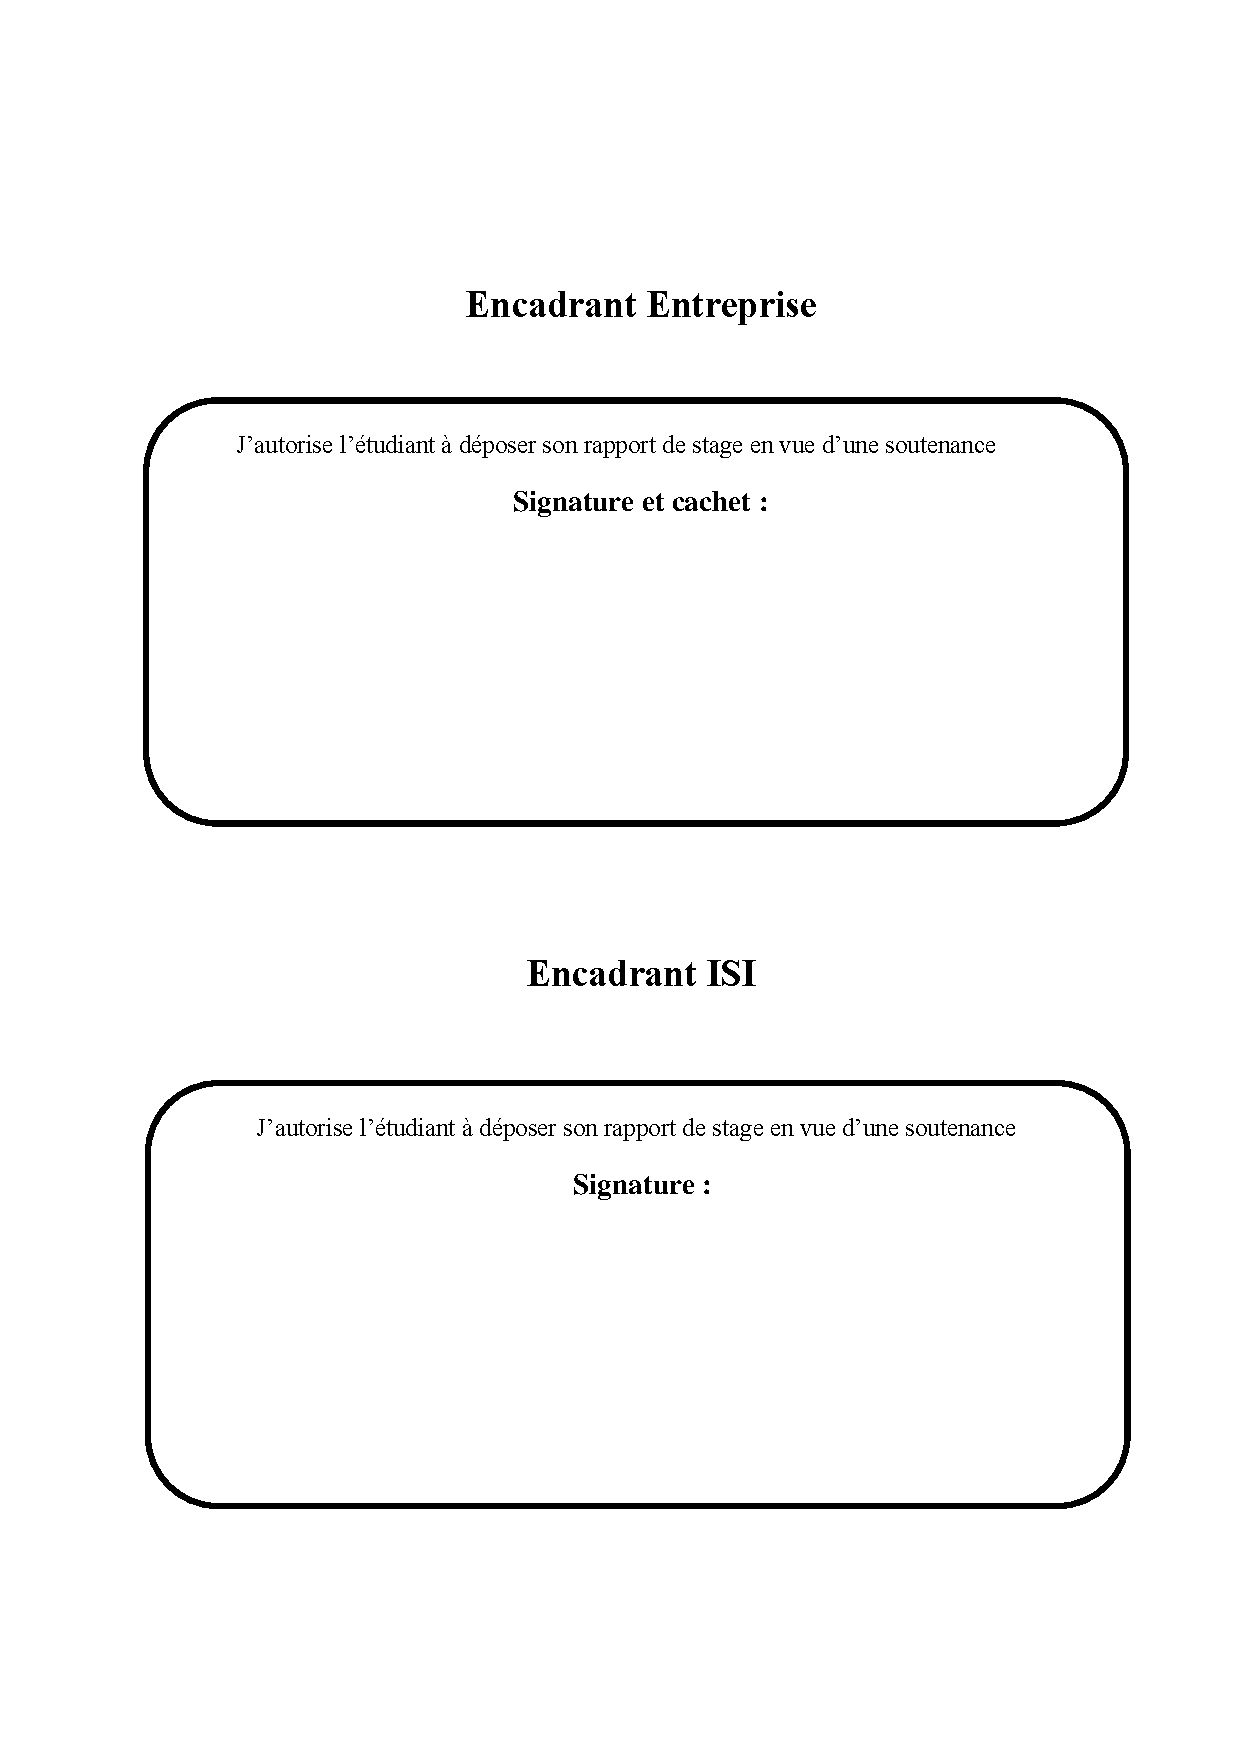
\includepdf{page_signature.pdf} 
\chapter{Dedication}
\vskip2.5cm
\thispagestyle{empty}
\begin{center}
 \emph{
 To my parents for their sacrifices, their encouragement throughout my studies, their patience and for the good values they have engraved in me. Thank you for everything you have done for me.\\To my family and friends for the encouragement and support you provided me through my many times of stress, excitement, frustration and celebration.\\To all of EY's family for the guidance, advice, and hospitality they provided. \\A special thanks to Mohamed Rezgui, Anis Hamdi, and Oussema Lessis for supporting and helping me during this whole process.\\To my faculty friends thank you for these amazing three years, it has been a blast.
 }
\vskip1cm

\hfill \textbf{Mohamed Baha Eddine Baghdadi\\}
\end{center}

\chapter{Acknowledgment}

 
Firstly, I would like to express my profound appreciation and gratitude to all those who supported me and provided me the possibility to complete and accomplish this project, I’m eternally grateful to all of you.\\

I would like to show my special and greatest appreciation to my Pedagogic adviser, Ms. Ben Youssef Nihel for her continuous support, patience, motivation, and immense knowledge. Her guidance helped me in all the time of the realization of this project and writing of this thesis. I could not have imagined having a better adviser and mentor. Thank you for believing in my potentials and for always pushing me to the limits and beyond.\\

My sincere thanks goes to Mr. Lessis Oussema and Mr. Dhifi Sami, who provided me with the opportunity to join their team as an intern. I am also grateful to all of EY’s family for creating a positive and comfortable work environment.\\

I acknowledge with much appreciation the jury members for honoring me by agreeing to evaluate this work.

\setcounter{secnumdepth}{3}
\setcounter{tocdepth}{2}
\tableofcontents


\listoffigures
\listoftables
\chapter*{Acronyms and Abbreviations}
\label{Intro}
\addcontentsline{toc}{chapter}{Acronyms and Abbreviations}
\markboth{Acronyms and Abbreviations}{Acronyms and Abbreviations}

\begin{acronym}\renewcommand{\\}{}
   \acro{API}{Application Programming Interface}
   \acro{APT}{Advanced Persistent Threat}
   \acro{CMD}{Command-Line Interface}
   \acro{CPU}{Central Processing Unit}
   \acro{CSRF}{Cross-Site Request Forgery}
   \acro{DF}{Digital Forensics}
   \acro{DFIR}{Digital Forensics and Incident Response}
   \acro{DLL}{Dynamic-Link Library}
   \acro{DOS}{Denial Of Service}
   \acro{EY}{Ernst \& Young}
   \acro{FTK}{Forensics Toolkit}
   \acro{GPS}{Global Positioning System}
   \acro{GUI}{Graphical User Interface}
   \acro{HTTP}{HyperText Transfer Protocol}
   \acro{IDE}{Integrated Development Environment}
   \acro{ISO}{International Organization for Standardization}
   \acro{JSON}{JavaScript Object Notation}
   \acro{LSASS}{Local Security Authority Subsystem Service}
   \acro{MITM}{Man In The Middle}
   \acro{MTV}{Model Template View}
   \acro{MVC}{Model View Controller}
   \acro{RAM}{Random Access Memory}
   \acro{RCE}{Remote Code Execution}
   \acro{SIEM}{Security Information and Event Management}
   \acro{UML}{Unified Modeling Language}
   \acro{UP}{Unified Process}
   \acro{VAD}{Virtual Address Descriptors}
   \acro{VM}{Virtual Machine}
   \acro{YARA}{Yet Another Recursive Acronym}
   
\end{acronym} 

\mainmatter
%%%%% Introduction

\chapter*{General Introduction}
\label{Intro}
\addcontentsline{toc}{chapter}{General Introduction}
\markboth{General Introduction}{General Introduction}
The reliance on technology nowadays for the public is implanted in the society. More activities and services are converting to the web each day that very few now can be performed without the use of digital devices. Most individuals and organizations have an electronic presence, using it to deliver services, communicate, plan meetings, play, socialize, and study. This advancement in technology means that most data is being digitized and devices are connected all over the world, making the spreading of data easier than before.\\
Digital devices like cell and smart phones, computers, and tablets store a lot of information relative to it's owner which makes it pretty inconvenient if it was stolen or hacked. These devices can be attacked as much as they can be part of a crime, be it a cybercrime or not. Considering the risks involved, companies have been investing a lot, these last few years, in the security of their information systems by seeking penetration testing services and implementing monitoring platforms like IDS, firewalls, and anti-viruses.\\
With the evolve of these technologies, engineers have to update and change their systems and tweak the products they implement per the company's needs, potentially leaving behind vulnerabilities that could be exploited. As no system is 100\% secure, incidents still occur, and organizations get hacked for various reasons.\\
The need for incident response and digital forensics has emerged, when a huge number of modern crimes where committed using computers and evidence was stored in there. Breached companies now hire professional investigators through consulting firms to assess the situation. A digital forensics investigation's goal is to determine the nature and events concerning a crime and locate the perpetrator by following an organized investigative procedure. The questions that drive a DF investigation are what happened, who did it, how and why it happened, and consulting firm like EY offer such security related services.\\
This project was implemented within the EY Advanced Cyber Security team. This team is a group of ethical hackers that offer consulting services to clients regarding information security. The team cover a variety of services such as external and internal penetration testing, code and configuration review, security audit, Red team services, and also Blue team services which contain precisely digital forensics investigation.\\
Facing the fact that modern computers have high specifications that require harder and longer processing, Data can get very large and can spread across devices, and malicious activities and programs are evolving in a way that they leave lesser trace by using volatile memory devices such as RAM rather than a hard disk. This means that the traditional computer forensic techniques and tools employed to an analyse a single device are no longer as effective. Investigations are even taking a move into using techniques like triage for the analysis instead of a full investigation of the E-evidence's data. This can lead into false negatives due to the human's fatigue and boredom when repeating such long tasks in the same way.\\
Therefore, a need to automate and simplify the process of forensic investigation is under the scope. This can be achieved by regrouping the traditional open-source tools into one platform and automating digital evidence processing, data extraction, and analysis. With such volumes of data, reduction of the data to be inspected into pre-selected categories is also important to keep a low false positives rate and rely on the investigator's judgmental decision as incident response should be no subject of doubt.\\
Correspondingly, this project is carried out as part of the preparation for the end-of-studies project presented for the National Diploma in Computing Science and Technologies in Network and Services Administration at the higher institute of computer science «ISI».\\
The project's objective is to achieve the development of the nonexistent platform for digital forensics regrouping tools and automating phases of various forensic analysis types for the investigation process as described above.\\
This report is organized as follows:
\begin{itemize}
    \item The first chapter introduces the host organization, in which the project has taken place. Then gives an overview on cybercrime and digital forensics methodology. And finally an analysis of existent solutions and our proposed solution.
    \item The second chapter presents the design phase of the project, identifying the specifications and introducing a set of diagrams.
    \item The third chapter describes the realization and implementation phase of the project, including the platform's architecture and tools used.
    \item The fourth chapter presents a case study using a real case scenario and the developed platform.
    \item Finally, we end our report with a general conclusion that summarizes the work we have accomplished and presents our outlook
\end{itemize}

%%%%% Chapter one

\renewcommand\thechapter{\Roman{chapter}}
\chapter{Project context and state of the art}


\newpage
\addcontentsline{toc}{section}{Introduction}
\section*{Introduction}
In This Chapter, we will give an overview of the host organization. Then we introduce cybercrime, hacking, and digital forensics, in the context of our project. Finally we will analyse and compare various existing solutions and present our proposed solution.

\section{Host organization}
\subsection{EY}
EY\cite{ey} is a multinational professional services organization that employs more than 270,000 professionals operating in over 700 offices in 150 countries, which makes its global reach enormous.\\
Some of the services it provides are audit, tax, business risk, technology and security risk services.\\
The objective of EY is to help clients, from start-ups to Fortune 500 companies, identify and capitalize on opportunities.\\
EY is a global leader in its areas of expertise, and is among the top four audit firms that have such a global coverage. These companies are referred to as the "Big Four", including KPMG, PricewaterhouseCoopers (PwC), and Deloitte.\\
The Tunisian experience began in 1987 with the creation of the AMC audit and advisory firm. In 1995, the company AMC became a member of Ernst \& Young's international network, becoming the only representative of the company in Tunisia.\\
To better understand the need and place of forensics in cyber security, we need to talk about cybercrime in general, how an attack happens, and what forensics has to do with it.
\subsection{EY Advanced Cyber Security Team}
EY Advanced Cyber security team is a group of highly qualified security consultants that are able to offer multiple services in cyber security. Below we list the main services that the team can provide:\\
\textbf{Infrastructure Security Assessment} services aim to provide accurate knowledge of the customer's level of security and to provide effective solutions to any weakness in their systems. This category includes traditional services such as ethical hacking, vulnerability assessment in different technology environments (wireless, VoIP, critical networks, Infrastructure) and technical review of IT policy compliance.
\begin{itemize}
    \item Internal Penetration Testing
    \item Wireless Security Assessments
    \item Operational Technology (SCADA) Penetration testing
    \item Smart Grid Penetration Testing
    \item Interactive Voice Response (IVR) System and VOIP security testing
    \item Network and System Infrastructure Configuration Reviews
    \item Virtual Desktop Infrastructure and Citrix Security Testing
    \item External Penetration Testing
\end{itemize}
\textbf{Application Security Solutions} area focuses on the security issues associated with the development of thick, mobile Web applications, poor application design, configuration, and implementation, which continue to be a major contributor to security breaches for organizations. For this, the team has qualified professionals in the field of application security, source code and application architectures.
\begin{itemize}
    \item Web Application and Web Services Testing.
    \item Dynamic Application Security Testing.
    \item Thick Application Testing.
    \item Mobile Application and Device Testing.
    \item Automated and Manual Source Code Review.
    \item Mainframe Infrastructure and Application Testing.
    \item Testing of ATM’s, ATM Switches, Check Processing Machines and POS Device Testing.
    \item Kiosk Testing.
\end{itemize}
\textbf{Red Team} services assess security controls related to defense in depth. They can range from targeted social engineering campaigns to simulated APT attacks. This service is designed to target organizations by prompting or manipulating personnel to provide sensitive information, bypass technical access controls on the network, or to gain unauthorized access to facilities. Red Team conducts these assessments from a variety of attack vectors such as phishing scenarios, USB attacks, specially crafted malware, and physical intrusions, all of which are associated with traditional penetration testing techniques. The goal is to compromise the network without the limitations of a traditional fixed scope like penetration testing.\\
\textbf{Security Training} provides a variety of custom security training courses that enable organizations to quickly, efficiently, and methodically train their personnel and developers to protect their environment and identify vulnerabilities in their information systems. The secure coding classes are designed to provide developers with the skills to develop and manage secure applications. In addition, it provides social engineering and physical security assessments to customers who require a comprehensive assessment of security posture encompassing non-technology assets such as human resources, processes, and organization. This team has successfully applied a risk-based approach to creating, executing, and implementing these types of large programs such as BAU (Business As Usual) audit-mandated, platform upgrade and major versions of high-risk, high-volume projects covering various clients and sectors.

\section{Preliminary study}
\subsection{Cybercrime}
'Cyber crime contains all criminal offences which are committed with the aid of communication devices in a network. this can be for example the Internet, the telephone line or the mobile network' (Wikipedia, 2008).\\
We can conclude that a cybercrime involves the use of digital device to attack another one on a specific network using some types of cyberattacks. The aim of a cyber attack is to steal, corrupt, or hack the information of an individual, an organization, or government office.\\
This is a process used to attempt accessing a system illegally to exploit unauthorized data or other information. This process involves the scanning of the Internet to find systems which could be mis-configured or contain security vulnerabilities. Once a cybercriminal gets access on a system, he can control the infected system and use it to spy on or disrupt services of other systems.\\
Cyber criminals can be anyone you may know or not know, like an annoyed employee, a partner, a competitor, an angry citizen, a terrorist or a bored teenager.

\subsection{Cyber attacks}
We will enumerate some of the most common cyber attacks that are seen daily.
\begin{enumerate}
    \item Phishing\\
    A phishing attack is a method by which an attacker makes himself look trustful so that a target shares his sensitive information thinking it's a legitimate service. These attacks can be seen in a form of an email, a phone call, or a website that tries to look legitimate. The name comes from the fact it's the same as catching fish, a hacker would use a website that looks like Paypal, for example, and lure the target into it so that he sends his personal and sensitive data, including credit card, home address, and phone number. An example overview of this attack type is shown in Figure I.1.
    \begin{figure}[H]
    \centering
    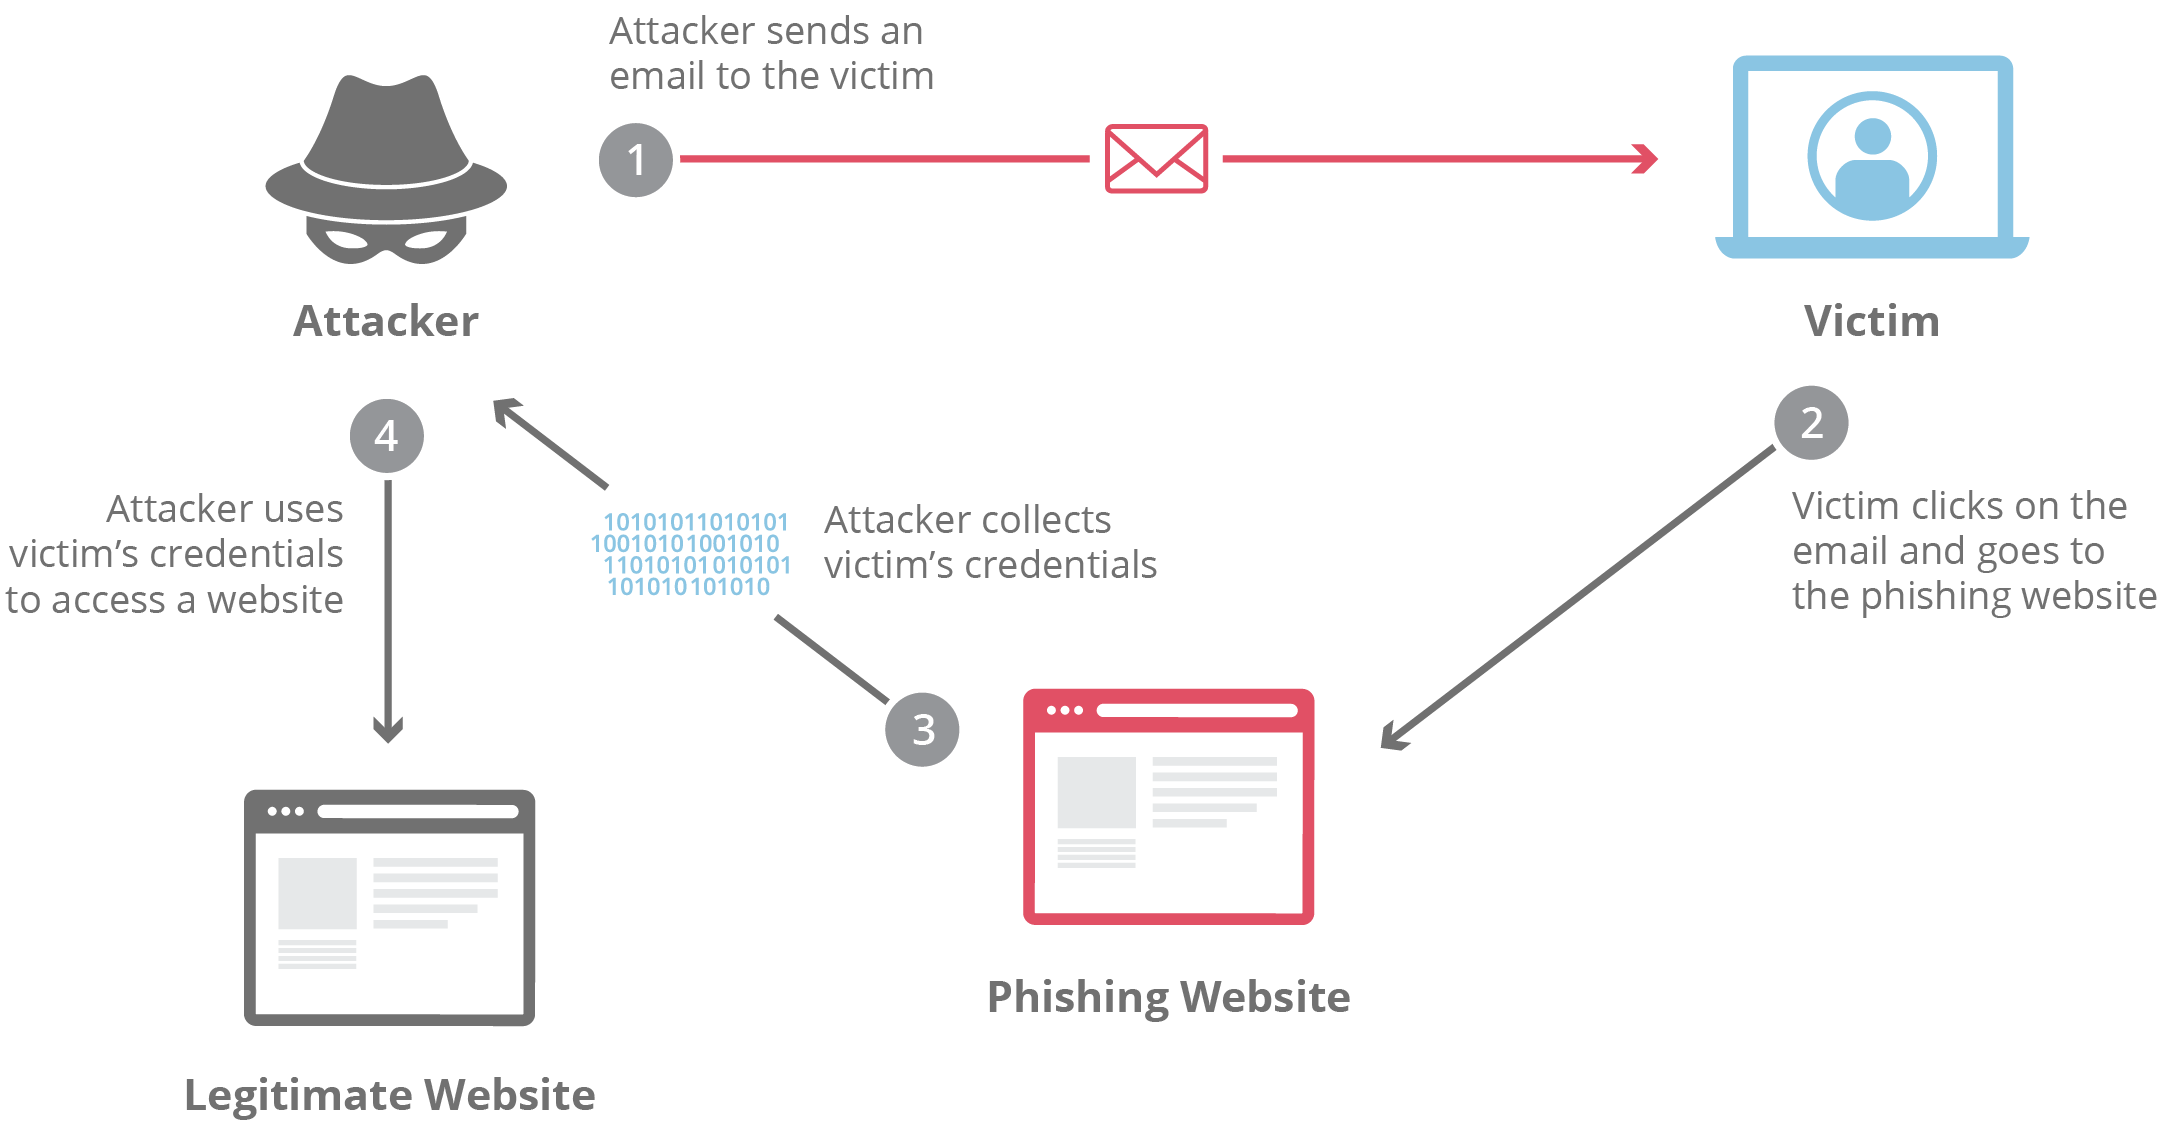
\includegraphics[width=0.7\columnwidth]{Figures/phising.png}
    \caption{Phishing attack \cite{phishing}}
    \end{figure}
    \item MITM\\
    A man in the middle attack is like eavesdropping but in a more advanced way. An attacker would be able to insert himself between two parties when communicating and all the conversation would run by him at first, which can be more understood from Figure I.2. This means that an attacker would actually know what was sent and received without both parties knowing anything about it. The attack can also be used to impersonate one of the parties and send a message from one party to another by signing it as one of them.
    \begin{figure}[H]
    \centering
    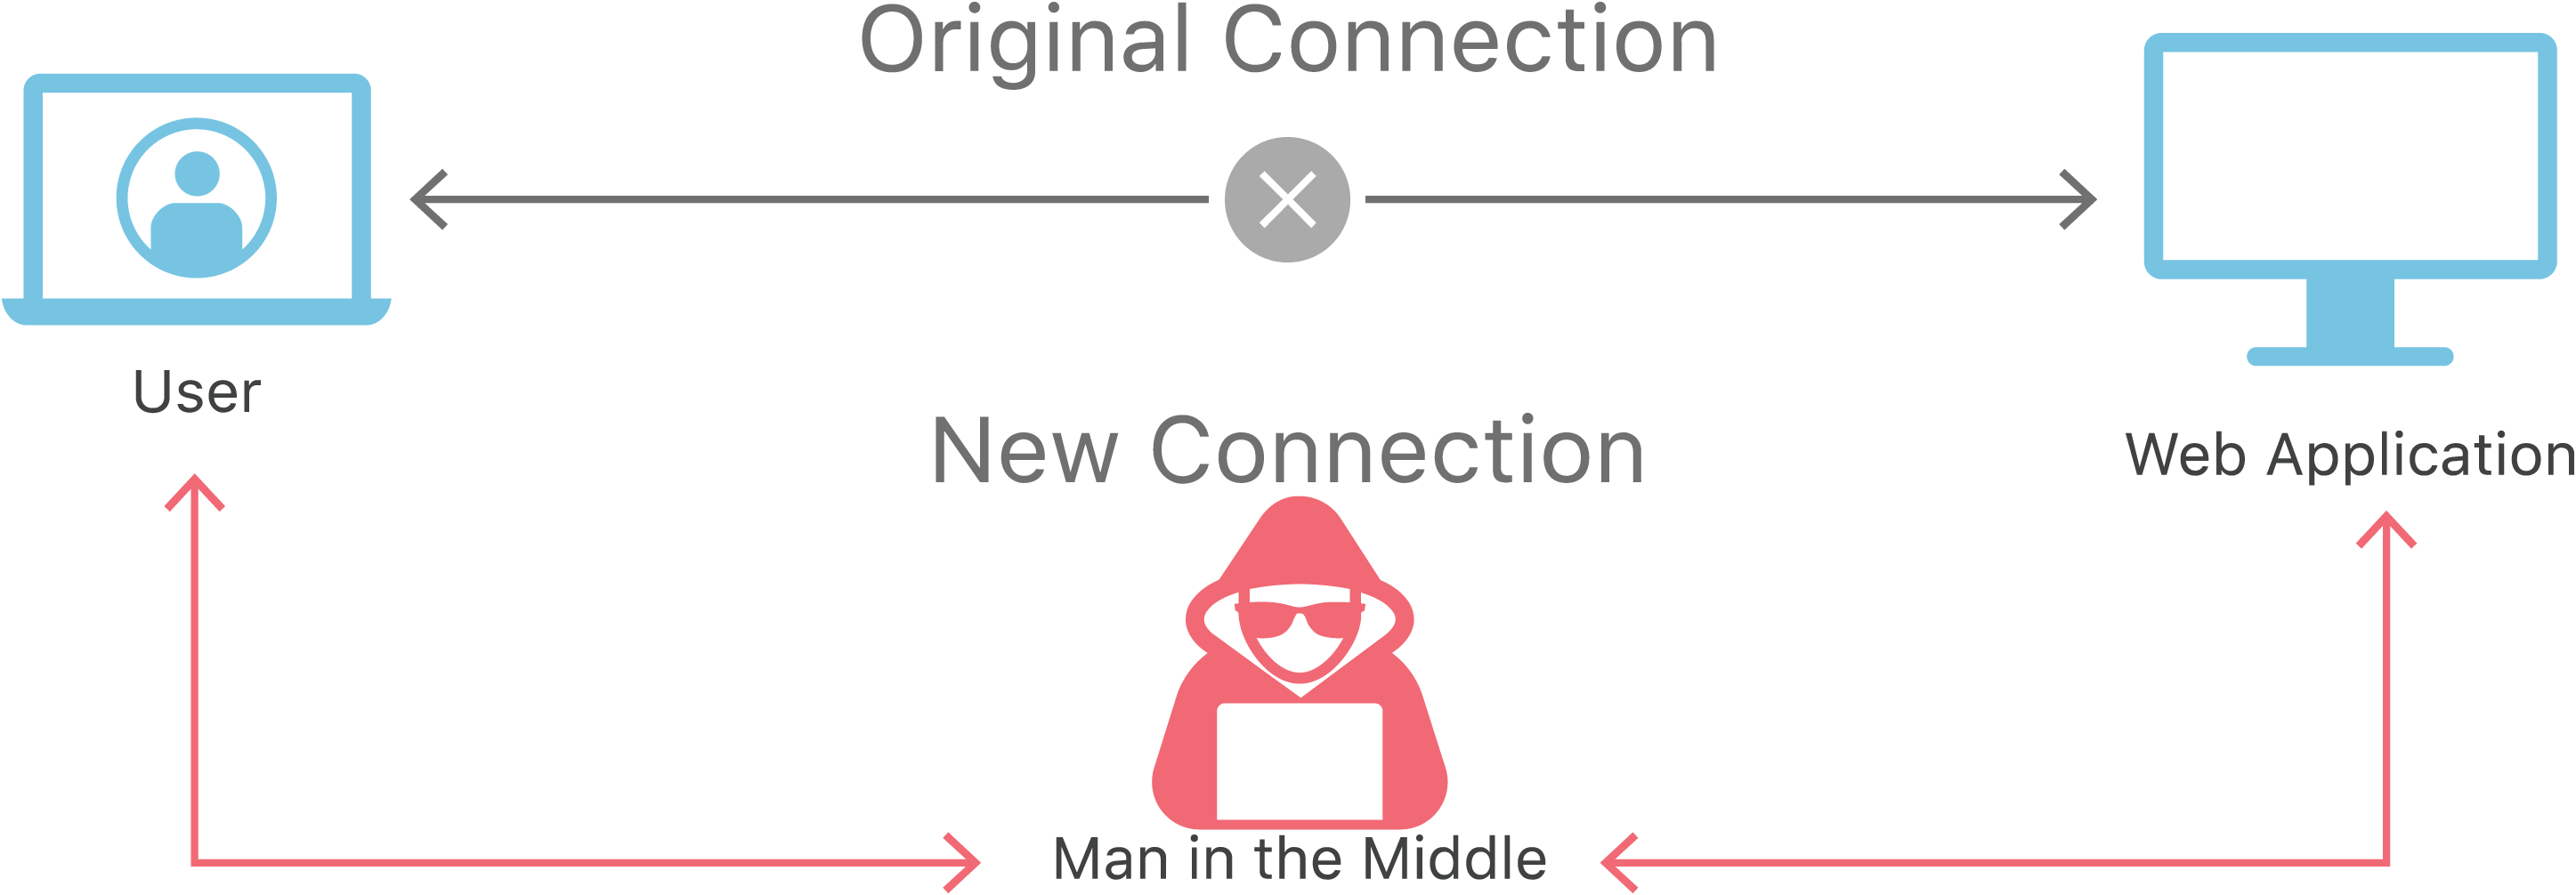
\includegraphics[width=0.7\columnwidth]{Figures/mitm.png}
    \caption{Man in the middle \cite{mitm}}
    \end{figure}
    \item DOS\\
    Denial of service attacks are used on networks and systems to render their services unavailable at a certain time or forever. The impact of such attacks is huge and mostly include economic and productivity losses at high expenses. DOS attacks are sometimes called DDOS (Distributed Denial Of Service), and that's when more than one computer is used in the process (most likely bots), as represented in Figure I.3. An example of how these attacks work can be by flooding the server with a number of requests that exceed the capability of it's buffer and render it unable to reply to normal requests, as follows:
    \begin{figure}[H]
    \centering
    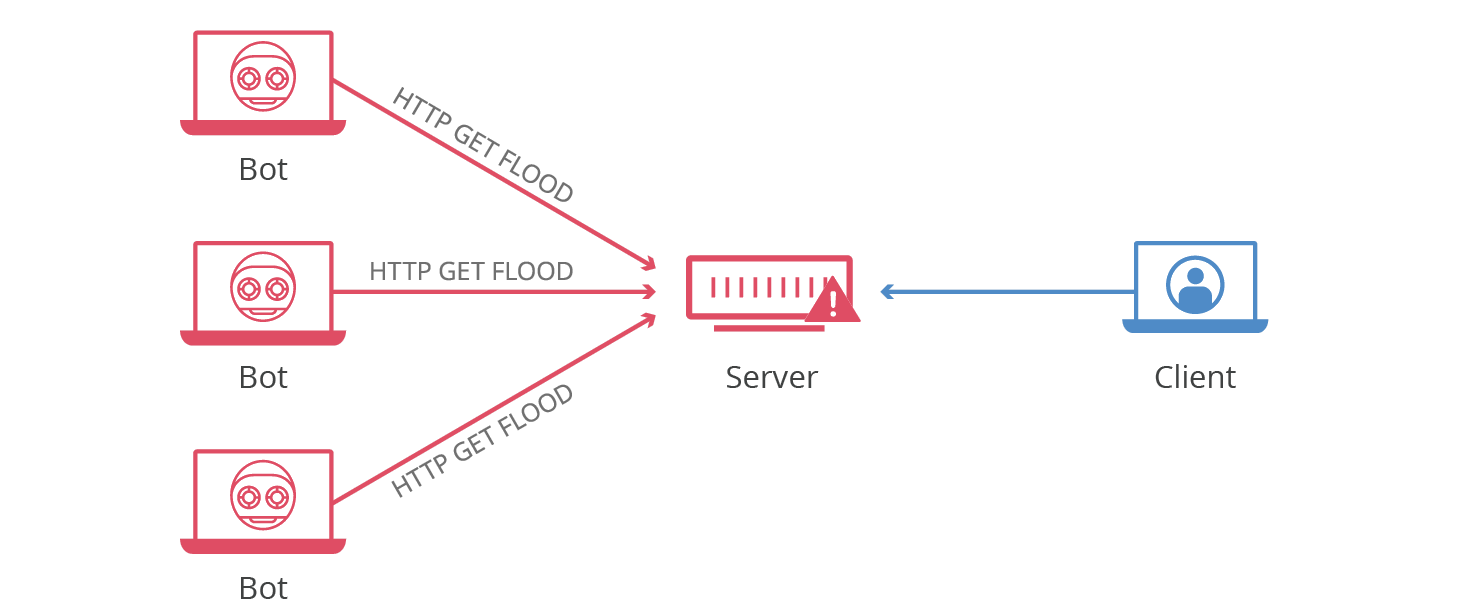
\includegraphics[width=0.8\columnwidth]{Figures/flood_ddos.png}
    \caption{DDOS - HTTP Flood Attack \cite{ddos}}
    \end{figure}
    
    
\end{enumerate}
\subsection{Malware}
A malware is basically any software that is harmful to an electronic device. This can help steal, corrupt, spy, and manipulate data on a computer without the knowledge of the owner.\\
Many types of malware exist. Some are more harmful and malicious than others. Most common type is encountered daily by all internet users, and that is Adware.

\textbf{Adware} are most know for the pop-ups they keep showing on a PC and websites you visit, offering free and exclusive experience like games, websites, and other matters. Figure I.4 shows an overview of what it looks like. It may not look that harmful and people may often leave it after failing to delete it since it doesn't pose a real threat more than a nuisance. But sometimes these software include Spyware or other type of malware that is activated as soon as you click on it.\\
\begin{figure}[H]
\centering
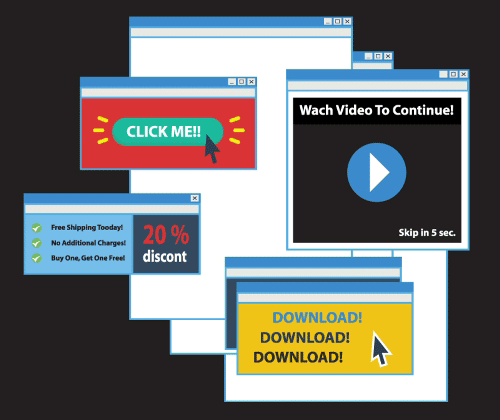
\includegraphics[width=0.5\columnwidth]{Figures/adware.png}
\caption{Adware overview \cite{adware}}
\end{figure}
\textbf{A Spyware} is installed on a host and hidden from the user. It is used to collect data like internet usage, keylogs, passwords, and personal information like we can see in the Hawkeye\cite{hawkeye} screenshot on Figure I.5. It then sends it to the attacker who keeps monitoring your PC this way without your knowledge. Another way to put such malicious software without being detected is integrating it within another legitimate software. In that case it's called a Trojan Horse.\\
\begin{figure}[H]
\centering
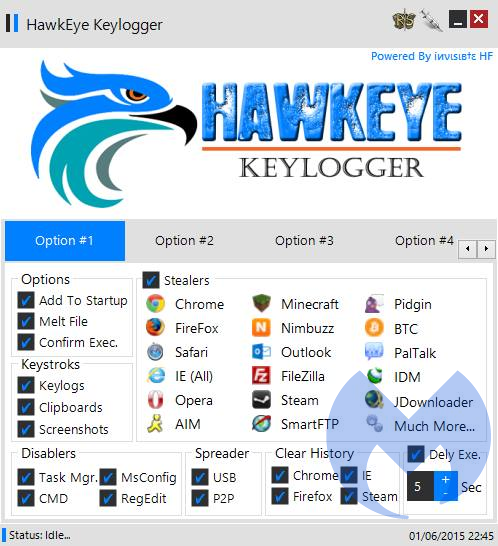
\includegraphics[width=0.6\columnwidth]{Figures/spyware.png}
\caption{Spyware Example \cite{spyware}}
\end{figure}
\textbf{A Trojan horse} is a type of malware that looks legitimate and eludes the user to trust it by pretending to be something the user wants. This software has some malicious code or function inside of it that isn't detected until it's running in the memory. As an example of how it is injected, Figure I.6 represents the Terdot trojan's initial injection chain. In most cases it can't be detected by signature because a good attacker would change variables and function names for each attack, making it have a new signature. While running in the background, a Trojan can install other malware like Ransomware.
\begin{figure}[H]
\centering
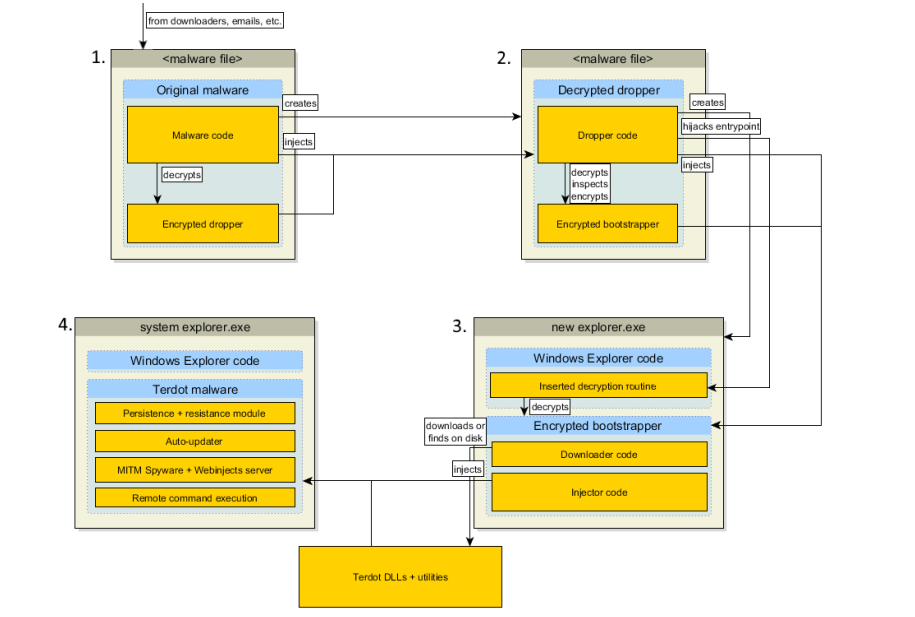
\includegraphics[width=0.6\columnwidth]{Figures/trojan.png}
\caption{Trojan injection process \cite{trojan}}
\end{figure}
\textbf{A Ransomware} is a malicious software that denies access to user's computer or data by encrypting or locking it and threatening to release is to the public or using it in illegal deals. The obvious way to get the data back is only if a ransom is paid to get the decryptor, but it surely doesn't guarantee that the attacker still has your data. The ransom is usually paid anonymously using cryptocurrency like Bitcoin. An example of a ransomware named Wannacry is shown on Figure I.7.
\begin{figure}[H]
\centering
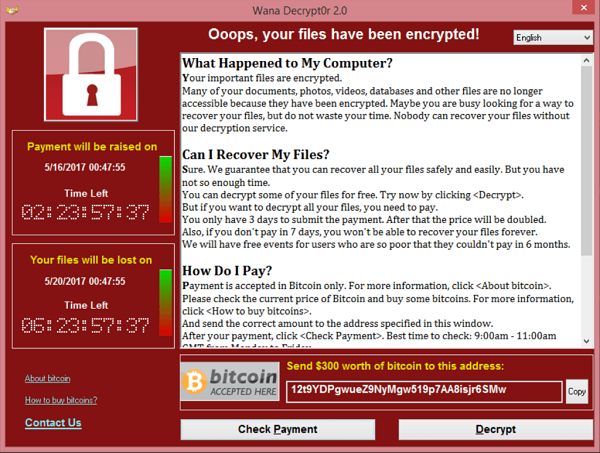
\includegraphics[width=0.7\columnwidth]{Figures/ransomware.png}
\caption{Wannacry ransomware example \cite{ransomware}}
\end{figure}



\subsection{Attack Phases}
There exists many tools that help blue teams to identify, hunt, and track suspicious activity in a network. No matter the steps taken by an attacker, his actions leave a corresponding artifact leaving behind footprints that can be critical. Attacks usually follow a predictable pattern, and we focus our first detection efforts on the set of fixed portions of that pattern.\\
For a better management and securing information systems, one must understand the attacker's view and steps. The phases on Figure I.8 are the 5 general steps a hacker would follow, from selecting his target, to owning the system.
\begin{figure}[H]
\centering
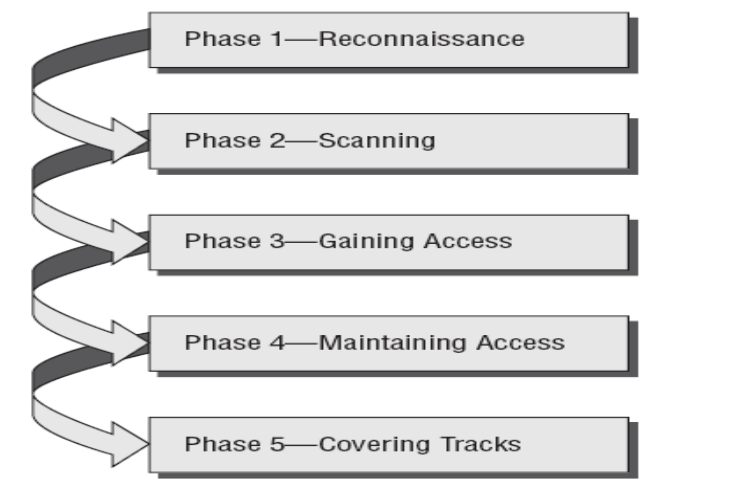
\includegraphics[width=0.6\columnwidth]{Figures/attack_phases.png}
\caption{Cyber Attack Phases\cite{attackphases}}
\label{fig_logo_utm}
\end{figure}
\subsubsection{Reconnaissance}
This phase requires the hacker to collect information about the potential victim. It involves identifying who the target is, and collecting information about it from public records, social media, website, etc. It also involves enumerating any parties involved with the target, like employees, associates, server hosts, previous breaches, etc.
\subsubsection{Scanning}
This phase involves active information gathering. An attacker would try to find out more information about the target by using port scanners, vulnerability scanners, and network scanners to determine any vulnerable data or service that could allow access to the target's machine or network.
\subsubsection{Gaining access}
Based on the collected information from the previous phases, the attacker plans on which attack vector he would go through to potentially have access. Attacks can vary from Social Engineering and Phishing, to exploiting a out-dated service or implementing a 0-day exploit.
\subsubsection{Maintaining access}
After getting access on a user's account in the system, the hacker would need to escalate his privileges to become an administrator and have the right to do anything he would like. The hacker will also need to deploy a backdoor in any form possible so that in case the attack was detected or that user's account got disabled, he would still have access to the network. This could happen by creating a new hidden user or allowing a service through the firewall.
\subsubsection{Clearing tracks}
All is done, The hacker has access and got what he wanted, now it's time to cover the tracks. The attacker will attempt to remove all tracks tracing him back to the attack. This phase is necessary so that no evidence is left for the forensics investigators to find in the system. This would require clearing out temporary files, logs, any data sent over the network, etc.

\section{Red Team}
\subsection{Introduction}
It is not enough to know the steps a hacker follows so we can secure the systems, detect his activities or track him down. The best way to secure your servers is to know it's weak points. Penetration testing allows us to know the vulnerabilities present on our systems and how they can be exploited so that we can take more defensive measures.\\
While Penetration Testing also involves testing for vulnerabilities in a system, network, or application to identify potential entry points for an attacker, it doesn't simulate a real hacking scenario.\\
When conducting a red team assessment, red teamers are required to replicate a real hacking scenario. Only a couple of people in the targeted firm would know about it, and most attack vectors are permitted. Thus, employing a red team assessment challenges a firm's detection and response capabilities effectively, touching most security policies and measures.\\
One of a red team's objectives is to get in without being detected, which involves hiding from defensive measures at first and then pass through the harder part which is not to be tracked down by the forensics investigators.
\subsection{Main Objectives}
\begin{itemize}
    \item Tests the effectiveness of an organization's digital forensics and incident response capability.
    \item Measures the capacity of the organization’s defensive posture.
    \item Provides access to good quality threat intelligence on an organization.
    \item Simulates a more realistic threat environment to the systems.
    \item Qualifies the effectiveness of an organization’s security awareness program.
    \item Ensures a way to build a proactive capability to manage and respond to real threats.
\end{itemize}

\section{Digital forensics}
\subsection{Introduction}
"DF is the scientific study of all the processes, involved in the recovery, preservation, and examination of digital evidence, including audio, imaging and communication devices" \cite{df}

A branch of forensic science that consists of identifying, preserving, recovering, analyzing and presenting facts about digital evidence found on computers or digital storage media devices. So it deals primarily with the recovery and analysis of latent evidence following cybercrimes or a service deficiency.\\
In most cases, an organization would conduct an investigation once a security breach has been detected, but it is essential that organizations take security measures and implement appropriate security policies and monitoring tools, as well as the identification and acquisition of live evidence right away in case of a suspected problem.\\
Computer forensics, or digital forensics in general, can mainly be about but is not limited to legal prosecution activities. A firm would conduct a forensics investigation for various reasons such as intelligence gathering, and finding the root cause of a server-side problem.\\
When being in the circle of attention, it is safe to say that any electronic device you touch will be used against you. Forensics investigations try to gather data from all places to acquire as much and efficient data as needed to prove a point. This is an immense field that is divided into more sub-fields.\\
We will now introduce some of the terms used in Digital Forensics for better clarification of future uses.
\begin{itemize}
    \item Cyber Forensics\\
    Investigative procedures used to collect, examine, analyse, and report findings associated with computing devices and networks, and is made suitable to enter such evidence into the court of law.
    \item Cyber Incident Response\\
    A methodical approach to managing a security breach with the intent of limiting damage, reducing recovery time, reducing costs, and developing a lessons-learned report. The lessons-learned report is used to stop or mitigate the impact of similar events as they occur in the future.
    \item E-evidence\\
    The forensics science involves collecting a set of evidence from a scene. Evidence deriving from any electronic source is called E-evidence.
\end{itemize}

\subsection{E-evidence sources}
E-evidence can be acquired from a lot of different devices. Each device has it's own specifications. We are to be focusing on computer forensics, as such, we shall present where we'll be getting evidence to be analysed later on.
\begin{itemize}
    \item Memory dump\\
    The memory data that sits on the Random Access Memory (RAM), should be retrieved immediately before anything due to the fact that it is volatile and would be lost in case of a system shutdown. This data contains the list of anything that was running or happened when the system was on. This list can include and is not limited to processes, internet browsing history, files accessed, network connection, logged in users and their hashes.
    \item Disk image\\
    Getting data from a non-volatile memory, which can be found on a computer’s hard disk drive, solid state drive, or external drive, would require keeping that drive for the whole investigation process or at least it's content. To keep that content as it is without keeping the hard disk, we need to take an image of it. A disk image is an exact copy of the contents on a hard drive and is stored on another device, and not stored on the hard drive from which the copy was made.
    \item Network traffic\\
    Network traffic is transmitted and then lost, so the analysis of this data is often pro-active, but we can record it using a network sniffer to analyse it at any other time. The traffic contains the list of packets transmitted through the network including connections made with other parties, protocols used, payloads sent and received. We can scan this data to potentially find malicious payloads that could be a cause of an attack or follow the identity of a possible attacker.
\end{itemize}

\subsection{Types of digital forensics}
Digital forensics involves the analysis of various hardware contents, each having it's own specifications. We will list and explain some of the most common types of forensic analysis.
\subsubsection{File system analysis}
File system forensics is the examination of storage devices like hard disks and USB sticks, in order to extract valuable information.\\
A disk contains all user files that could contain a lot of evidence and logs to help us later on in the analysis. We could also recover deleted files, metadata and sessions from different systems.

\subsubsection{Memory analysis}
Memory forensics refer to the analysis of volatile data from a computer which is exported into physical file dump.\\
Since everything that happens on a computer passes through the RAM first, like opened files, programs (processes), and network connections, we need to dump and analyse it in order to understand what happened on the system when it was up.\\
That is why new attacks use techniques that leave no traces on disk but only on live memory since it will be lost later.

\subsubsection{Network analysis}
Intrusion detection systems will play a key role as input data sources for network forensic analysis into the foreseeable future. This is especially true because they are very commonly used methods of capturing data from a wide variety of digital sources and storing that data in a centralized repository that could be made accessible to analytical processes with forensic objectives.\\
Performing network forensic analysis will require critical observance of large amounts of highly filtered data from varying sources, many times over large geographic spaces. This complexity causes concerns in related matters like how often the data or snapshots are to be collected, who is to collect the data, since it needs to be taken immediately, and there needs to be certain level of trust in that party, and what exactly is to be collected and what to filter out.

\subsubsection{Mobile analysis}
Mobile device analysis relates to the recovery of digital evidence or data from a mobile device.\\
An estimated 66.7\% of the population worldwide owns a cellphone by now. This increases the probability that if a certain person is involved in a crime or an anomaly that happened to a system, we would find some data referring to it somewhere in his mobile devices. Although that probability may not be high enough, but it's getting higher since a modern human's mindset would require him to at least plan it on an electronic device.\\
Data recovered from these devices can be pretty helpful. We could recover GPS-saved location history, call logs, contacts, images taken by the user and even the deleted one's.

\subsubsection{Log analysis}
Log analysis is actually one that we talk about the least, but end up doing the most. SIEMs were supposed to keep us from needing to do this, but a good way to understand exactly what happened is to keep reading the logs from the system and software affected. Analyzing log falls into system anomalies detection, in most cases. Since services and implemented monitoring solutions keep track of every action that takes place on a system, it is inevitable to produce a timeline through the logs to understand where something went wrong and follow it to the root cause.

\subsection{Digital forensics models}
Digital forensics is part of a security approach. It can help with the after-incident, but has also evolved to deal with detected attacks or crimes on the go. These approaches are known as Reactive and Proactive forensics.
\subsubsection{Reactive}
This is the traditional or post-mortem approach of investigating a digital crime after an incident has occurred, which we will research more for the purpose of this report. This involves identifying, preserving, collecting, analyzing, and generating the final report. Two types of evidence are gathered under this component:
\begin{itemize}
    \item Active: Active evidence refers to collecting all live (dynamic) evidence that exists after an incident. An example of such evidence is processes running in memory.
    \item Reactive : refers to collecting all the static evidence remaining, such as an image of a hard drive.
\end{itemize}
\subsubsection{Proactive}
Proactive Digital Forensic Component has the ability to proactively collect data, preserve it, detect suspicious events, gather evidence, carry out the analysis and build a case against any questionable activities. In addition, an automated report is generated for later use in the reactive component. The evidence gathered in this component is the proactive evidence that relates to a specific event or incident as it occurs.\\
As opposed to the reactive component, the collection phase in this component comes before preservation since no incident has been identified yet. This approach is also more useful for detecting attacks using Anti-Forensics.


\subsection{Anti-Forensics}
The term anti-forensics refers to methods that prevent forensic tools, investigations, and investigators from achieving their goals. Any methodologies that used to incriminating computer forensic process can be considered as a anti forensic. Basically, there are four types of anti forensic technique such as destruction, evidence source elimination, evidence hiding, and evidence counterfeiting.. From a digital investigation perspective, anti-forensics can do the following:
\begin{itemize}
    \item Prevent detection of digital crime.
    \item Provide misleading evidence that can jeopardize the whole investigation.
    \item Prevent evidence collection.
    \item Obfuscate data that could lead to evidence.
\end{itemize}

\subsection{Stages of digital forensics}
The traditional digital forensics follows the reactive model which consists of 5 stages followed by investigators to conduct the investigation. These stages can be named, described, or grouped otherwise, so we are following the steps of a DF handbook\cite{handbook} as presented in Figure I.9.
\begin{figure}[H]
\centering

\includegraphics[width=1\columnwidth]{Figures/foren.png}
\caption{Digital forensics process}
\end{figure}
\subsubsection{Preserve}
This is a fundamental element in all digital forensics activities. If potential evidence is not preserved in the correct manner, then it may have little or no value in any criminal or civil proceedings, although it may still be useful for gathering basic information about a case. The preservation of evidence must be conducted by staff that acquire the skills and techniques required and use of the appropriate tools to preserve the evidence in an unaltered state. Developed and tested procedures that are known to be accepted by the courts should be followed whenever possible. The preservation of evidence is most important and must be considered at all stages of the investigation.
\subsubsection{Collect}
The collection of any digital device or information that may be used as evidence must be carried out by trained staff and must follow specific procedures so that its value as evidence is preserved for the analysis and usage in any legal or disciplinary proceedings.
\subsubsection{Examine}
The examination of evidence must be carried out using tools that have been tested or accepted by the courts as providing information in a faithful form. Any data produced for the purposes of proof must be reproducible by another investigator. The examination of the evidence must be thorough and in a comprehensive manner. The examination of the evidence should, as far as possible, focus on an image of the original material rather than on the original material itself, although it is recognized that, in exceptional circumstances, this might not be possible.
\subsubsection{Analyse}
Evidence analysis is the forensic phase in which the information held and examined is interpreted as allowing conclusions to be drawn and the truth about what happened during and before an incident. This will normally be done in the computer forensics lab and care should be taken to ensure that any results are documented and can be recreated by another investigator.
\subsubsection{Present}
The presentation of the results of the analysed data is as important as any other phase of the DF process. If the results are not presented in a coherent, comprehensive and credible form, the efforts made in the previous phases will have been in vain.


\section{Study of the Existing Solutions}
This section presents a study of the most popular existing digital forensics tools. We tried to classify and compare them to each other, and conclude their limits to finally present our proposed solution.
\subsection{Analysis of the Existing Solutions}
DF is one of the most complex science fields. It requires attention and precision in most of it's phases, that following all of them manually would not get the job done. A lot of tools started to appear, each tool simplifies one of the processes and they hardly regroup more than one phase due to the sub-processes in each of them. Most DF tools simplify a set of steps rather than automate a whole process but it's been very useful.
\subsubsection{Description of the most popular solutions}
This section covers a large number of penetration testing tools ranging from free open source software to commercial ones.
\begin{enumerate}
\item \textbf{Volatility} \\ Open-source memory analysis tool which could extract useful data like processes and network connections from memory dumps. Volatility is widely used when analyzing memory dumps, but requires an experienced investigator to know the plugins to be used and regroup the acquired data to then analyse it efficiently.
\item \textbf{Rekall} \\ An open-source memory analysis tool that was historically a fork of the Volatility memory analysis framework and is now more advanced, that it comes with a complete platform for acquisition and analysis.
\item \textbf{Encase} \\ A software that allows the investigator to conduct in depth analysis of user files to collect evidence from a seized hard drive such as documents, internet history and Windows Registry information. Encase is a professional software that can be really expensive depending on which product is needed.
\item \textbf{FTK} \\ Software package developed by AccessData. It enables the acquisition, analysis and extraction of multiple data from a computer disk, such as deleted files and text search. The set of tools in FTK are handful when acquiring dumps of live memory or hard disk, and getting information out of it.
\item \textbf{NIKSUN NetDetector} \\ 
A full-featured appliance for network security surveillance, anomaly detection, and forensics. It complements existing network security tools, such as firewalls, IDS, and IPS. NetDetector should be installed before-hand to detect threats and log connections. The price for NetDetector is rather high but is relevant for the tasks it accomplishes when used correctly.
\item \textbf{NetworkMiner} \\ 
A network analysis tool developed for windows which is available in free and professional edition. It is used to analyse network traffic and allow regenerating files and data transmitted through that traffic.
\end{enumerate}
\subsubsection{Comparison between the studied solutions}
Each one of the tools mentioned specifies in a certain category. But we will try to compare them based on the phases and options they can provide. 
 Table \ref{tab_val} presents a comparison between the existing Penetration testing platforms.
\begin{hyphenrules}{nohyphenation}
\begin{table}[H]
\caption{Comparison between the studied solutions}
\centering
\begin{tabular}{|>{\columncolor[gray]{0.9}}p{2.5cm}|p{2cm}|p{1.8cm}|p{1.8cm}|p{1.8cm}|p{2.3cm}|p{2.3cm}|}
\hline
\textbf{} & \cellcolor[gray]{0.9}\textbf{Volatility} & \cellcolor[gray]{0.9}\textbf{Rekall} & \cellcolor[gray]{0.9}\textbf{EnCase} & \cellcolor[gray]{0.9}\textbf{FTK} & \cellcolor[gray]{0.9}\textbf{Net Detector} & \cellcolor[gray]{0.9}\textbf{Network Miner} \\ 
\hline 
Memory Forensics & \cellcolor{green!25}YES & \cellcolor{green!25}YES & \cellcolor{green!25}YES & \cellcolor{red!25}NO & \cellcolor{red!25}NO & \cellcolor{red!25}NO \\ 
\hline
Disk Forensics & \cellcolor{red!25}NO & \cellcolor{red!25}NO & \cellcolor{green!25}YES & \cellcolor{green!25}YES & \cellcolor{red!25}NO & \cellcolor{red!25}NO \\ 
\hline
Network Forensics & \cellcolor{red!25}NO & \cellcolor{red!25}NO & \cellcolor{red!25}NO & \cellcolor{red!25}NO & \cellcolor{green!25}YES & \cellcolor{green!25}YES \\ 
\hline
\hline
Acquisition & \cellcolor{red!25}NO & \cellcolor{red!25}NO & \cellcolor{green!25}YES & \cellcolor{green!25}YES & \cellcolor{green!25}YES & \cellcolor{red!25}YES \\
\hline
Analysis & \cellcolor{green!25}YES & \cellcolor{green!25}YES & \cellcolor{green!25}YES & \cellcolor{green!25}YES & \cellcolor{green!25}YES & \cellcolor{green!25}YES \\ 
\hline
Reporting & \cellcolor{red!25}NO & \cellcolor{red!25}NO & \cellcolor{red!25}NO & \cellcolor{green!25}YES & \cellcolor{red!25}NO & \cellcolor{red!25}NO \\
\hline
Cross-platform & \cellcolor{green!25}YES & \cellcolor{green!25}YES & \cellcolor{green!25}YES & \cellcolor{red!25}NO & \cellcolor{green!25}YES & \cellcolor{red!25}NO \\ 
\hline
Swap analysis & \cellcolor{green!25}YES & \cellcolor{green!25}YES & \cellcolor{red!25}NO & \cellcolor{red!25}NO & \cellcolor{red!25}NO & \cellcolor{red!25}NO \\ 
\hline
\end{tabular}  
\label{tab_val}
\end{table}
\end{hyphenrules}
\subsubsection{Limits of the Existing solutions}
Conducting a digital forensics investigation requires expertise in the attack and defense fields and expertise in the forensics science, which would be hard and boring, at some point, without automating some of the steps included in these investigations. That is why some organizations opt to buy highly expensive software that can do some of the work in one of the different investigation phases, but not all of them.\\
The reality is that no one tool does it all. Most software touch only one category and no more than two phases, and are also sold with a very high expense. As a consequence, budget permitting, labs need to have a variety of tools available. These software can bring some capabilities to the table, that general-purpose tools don't offer, but should be used mostly in law enforcement forensics labs.\\
All of this led to our solution that supports and combines different forensic analysis types while including some open-source tools and extracting data in all at once using these tools automatically, which we will get to in the next section.

\subsection{Proposed Solution}
Using a lot of tools that require a lot of dependencies and handling can be tiring, especially the first couple of steps when extracting and visualizing acquired data before proceeding to analysis and detection of problems or anomalies, finding a culprit, or following and understanding the footsteps of an attacker.\\
The consultant will be required to acquire digital evidence, and extract the most out of it, leading to an explanation of what happened, how it happened, and why it happened.\\
Like any other process in the information security field, it needs intelligence, observance and concentration to reverse engineer an attack. Following that, automated digital forensics has received a lot of criticism from professionals for that it can't detect a large variety of vectors even when considering dynamic forensics using artificial intelligence. However, critics also currently accept a certain level of automation to help them in their daily tasks.
Manually extracting processes and files and comparing them and scanning each one alone is impractical. We can confirm that automating certain phases in computer forensics would assure:
\begin{itemize}
    \item  Increasing productivity by reducing the time taken to perform repetitive tasks.
    \item  Ensuring that main tasks will run effortlessly and the same way every time it is run.
    \item  A seamless platform integrating your needs.
\end{itemize}
In order to achieve our objectives, we propose to develop a platform that consolidates most useful computer forensics tools and can automate the regroup, summarizing of useful extracted data, and automatic identification of issues given a certain evidence file, which could be a memory dump, network flow, or disk image. This will allow to react better, more intelligently, and possibly fix your next step in the analysis.\\
Some of the function the platform will take care of are these:
\begin{itemize}
    \item Extraction of processes and running them through YARA rules, from memory dumps.
    \item Listing Internet activity, files, GUI, from memory dumps.
    \item Extraction of logs, deleted files, and media, from disk images.
    \item Summarizing network connections and extraction of files in network traffic.
    \item Detection of common suspicious activities.
    \item Detection of malware, keyloggers, and suspicious connection.
\end{itemize}
Our solution also focuses on fixing two problems in today's digital forensics tools:
\begin{itemize}
    \item They were designed to help investigators find specific pieces of evidence, not to assist them in investigations.
    \item They were designed to solve crimes against people where the evidence is digital, not to assist in solving crimes committed with or against computers.
\end{itemize}
\addcontentsline{toc}{section}{Conclusion}
\section*{Conclusion}
Throughout this chapter, we introduced the host organization in which the project was developed and maintained. We then presented a theoretical research on cybercrime and digital forensics. We have also mentioned and compared some of the different solution used by digital forensics investigators. Finally, we introduced our solution and project objective. This chapter allows us to understand the needs and limitations that we need to overcome, which will lead to understanding the platform's requirements that we will analysis in the next chapter.

%%%%% Chapter two
\renewcommand\thechapter{\Roman{chapter}}
\chapter{Requirements analysis and specification}
\newpage
\addcontentsline{toc}{section}{Introduction}

\section*{Introduction}
In this chapter, we will present our development methodology. Then we will identify the main actors involved in our platform, and analyse the functional and non-functional requirements. We will then present and describe the use cases most relative to the project's objective. Finally, we will present the sequence diagrams of the platform.

\section{Work methodology}
This section's aim is to explain our methodological approach regarding the development process and the chosen modeling language.
\subsection{Development process}
We chose the Unified Process (UP) to carry out this project, as it allows us to monitor progress in terms of time, cost, quality and client satisfaction. This process is an incremental, iterative process that is based on the system architecture.\\
The unified process is done in four phases: inception, elaboration, construction and transition. Each phase repeats a series of iterations a number of times where each iteration is composed of five activities: capturing needs, analysis, design, implementation, and testing.
\begin{figure}[H]
\centering
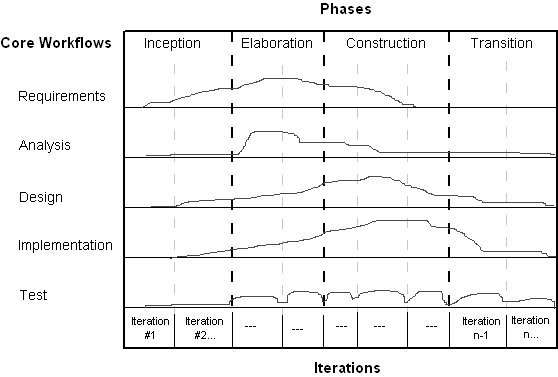
\includegraphics[width=0.7\columnwidth]{Figures/methodo.png}
\caption{Unified process life cycle\cite{methodo}}
\end{figure}
\begin{itemize}
    \item \textbf{Inception}\\
    This is the first phase of the unified process. It is a question of delimiting the scope of the system, meaning, to detect what must appear inside the system and what must remain outside, to identify the actors, to remove any inexactness about the necessary needs and requirements in this phase. It is also a matter building an architecture capable of functioning. In this phase, it is also useful to identify any critical risks that are likely to jeopardize the smooth progress of the project.
    \item \textbf{Elaboration}\\
    After understanding the system, clearing the initial features and functions, specifying the risks, the work to be done now is to stabilize the architecture of the system. This involves refining the initial use case model, even capturing new needs, analyzing and designing most of the use cases formulated, and possibly implementing and testing those initial use cases.
    \item \textbf{Construction}\\
    In this phase we have to try to capture all the remaining needs as it is practically impossible to do in the next phase. Then continue the analysis, design and especially the implementation of all use cases and other diagrams' contents. At the end of this phase, developers must provide an executable and ready version of the system.
    \item \textbf{Transition}\\
    This is the phase that finalizes the product. During this phase, it is necessary to check if the system fully offers the services requested and required by the users, to detect defects, to fill in the gaps in the documentation of the software and to adapt it to the final environment.
\end{itemize}

\subsection{Modeling language}
For a steady and organized application, after choosing the methodology, we need to design our platform using an efficient modeling language. Our choice was Unified modeling language (UML). UML is a language that aids in modeling different artifacts of a system which details the possible scenarios and solutions of our problem.

\section{Actors identification}
Before looking at the platform requirements, we will list the main actors involved. In our case, there are two actors since the platform is used for analysis only.
\begin{itemize}
    \item \textbf{Administrator:}
    This actor has full control over the platform. His role is to manage the users and platform environment. He can add and remove users, update user information or change a user into an admin, manage disk usage, and view logs.
    \item \textbf{Consultant:}
    This actor is an EY employee from the Advanced Cyber Security Team. He gets to analyse E-evidence, using the platform, by providing a file and other information, and can view the results.
\end{itemize}

\section{Requirement specification}
Here we will introduce the platform's different functional and non-functional specifications.
\subsection{Functional specification}
The platform must offer the users the following functions:
\begin{itemize}
    \item \textbf{Authenticate:} Authenticate using credentials.
    \item \textbf{Manage cases:} Add a new case to be analysed, remove existent cases, and consult the list of cases previously added.
    \item \textbf{Check case status:} Check if case is being analysed, done, or unsupported.
    \item \textbf{View case analysis:} Choose a case that is ready and view the analysis reports generated in the platform.
    \item \textbf{Consult administration dashboard:} View admin dashboard that shows general platform information. This function requires the user to be an administrator.
    \item \textbf{Manage Consultants:} Allow an administrator to add, remove or change a consultant's information and role.
    \item \textbf{View session log:} An administrator should be able to View lastly added and removed cases.
    \item \textbf{Logout:} A link to close the current user session.
\end{itemize}
The platform must be secure against the following:
\begin{itemize}
    \item \textbf{Unauthenticated access:} Users must be logged-in to access and use the various platform pages.
    \item \textbf{Unauthorized access:} Users must have access restrictions based on their type, group, or content created.
    \item \textbf{Remote Code Execution:} The application should not be vulnerable to remote code execution through the various commands it uses.
\end{itemize}
\subsection{Non-Functional specification}
Non-functional specifications describe the attributes of the application. In our platform, we have mainly:
\begin{itemize}
    \item \textbf{Availability:} The platform should be accessible when the user needs it.
    \item \textbf{Usability:} The platform must have a user-friendly interface.
    \item \textbf{Performance:} The platform should have quick response time.
    \item \textbf{Portability:} The platform should be easy to move and install on other machines.
\end{itemize}

\section{Platform Design}
This section presents the different UML diagrams modeled to define the platform.
\subsection{Use Case Diagrams presentation}
We will now model the different specifications mentioned earlier using Use Case diagrams. A use case diagram represents a user’s interaction with the system and make it possible to highlight the need of the system user, thus, we will present the most important use cases.\\
But first we will give an overview of the whole application in Figure II.1.
\begin{figure}[H]
\centering
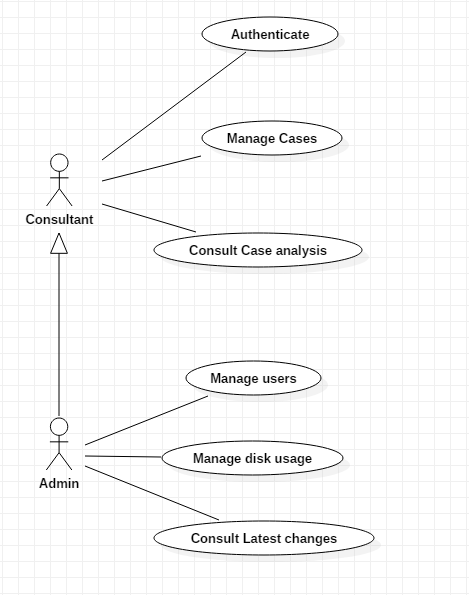
\includegraphics[width=0.6\columnwidth]{Figures/usecase.png}
\caption{Global use case}
\end{figure}
\subsubsection{Case management and analysis}
Figure II.2 shows that an authenticated consultant would be able to use the platform to do the following:
\begin{itemize}
    \item Add a new case: The user will need to provide an evidence file to scan and choose a type of forensics to apply.
    \item Remove a case: The user will be able to select an existent case to be deleted.
    \item Consult case analysis: The user will be able to see reports of extracted data from the provided evidence file regarding the selected case, after the analysis is complete.
\end{itemize}
\begin{figure}[H]
\centering
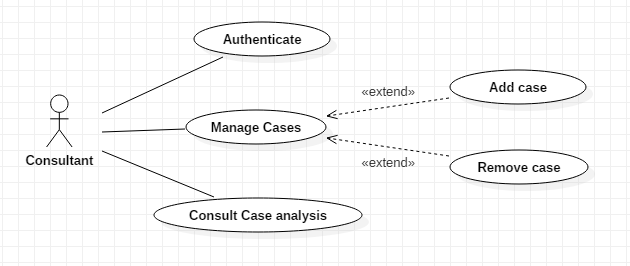
\includegraphics[width=1\columnwidth]{Figures/usecase1.png}
\caption{Case management and analysis use case}
\end{figure}

\subsubsection{Administration}
An Authenticated Administrator, as explained in Figure II.3, would be able to use the platform as an investigator, but also has a unique dashboard that allows him to:
\begin{itemize}
    \item Add a new user: The admin can create a new account for an investigator and fill in his details.
    \item Remove a user: The admin can delete a user account from the platform.
    \item Edit a user: The admin can change a user's account general information or password.
    \item Consult disk usage: The admin, based on the volume used by the application, can choose to clear up space by deleting files from already-analysed cases and temporary files.
    \item Consult log: The admin can see latest changes made in the platform by other users.
\end{itemize}
\begin{figure}[H]
\centering
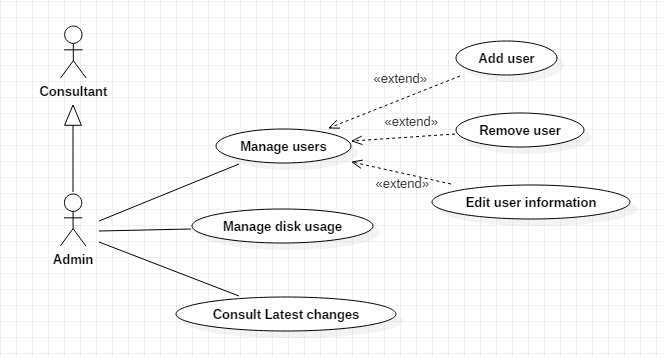
\includegraphics[width=1\columnwidth]{Figures/usecase2.png}
\caption{Administration use case}
\end{figure}

\subsection{Textual description of use cases}
Use case diagrams are useful to give an overview and visualize the interaction between the users and the system, but we also need to give more details about each use case through textual description represented in both Table II.1 and Table II.2. 

\newpage
\begin{longtable}{|p{15cm}|}
\hline
\multicolumn{1}{|c|}{\textbf{Administration use case textual description}}\\
\hline
\multicolumn{1}{|l|}{\textbf{Actor:} } \\
\quad Administrator \\
\multicolumn{1}{|l|}{\textbf{Summary:} } \\
\quad This use case allows the administrator to manage some platform options and the user accounts in it.\\
\multicolumn{1}{|l|}{\textbf{Preconditions:} }\\
\quad Authenticated administrator.\\
\multicolumn{1}{|l|}{\textbf{Scenario:}} \\
\quad - The administrator signs in using his username and password. \\
\quad - The administrator is able to manage cases as a consultant himself. \\
\quad - The administrator views and clears disk usage. \\
\quad - The administrator views the number and the list of users, adds a user, selects a user to change his information or remove him. \\
\quad - The administrator views the latest changes made to the platform by other users. \\
\multicolumn{1}{|l|}{\textbf{Exceptions:}} \\
\quad E1 : incorrect login credentials.\\
\quad 1) The system reloads the login page.\\
\quad E2 : invalid new user information.\\
\quad 2) The system reloads the user modification page.\\
\hline
\caption{\mbox{Description of the "Administration" use case}}
\end{longtable}

\newpage
\begin{longtable}{|p{15cm}|}
\hline
\multicolumn{1}{|c|}{\textbf{Case management and analysis textual description}} \\
\hline
\multicolumn{1}{|l|}{\textbf{Actor:} } \\
\quad Consultant\\
\multicolumn{1}{|l|}{\textbf{Summary:} } \\
\quad This use case allows the consultant to create a new case to analyse an E-evidence, and manage old cases.\\
\multicolumn{1}{|l|}{\textbf{Preconditions:} }\\
\quad Authenticated consultant.\\
\multicolumn{1}{|l|}{\textbf{Scenario:}} \\
\quad - The consultant signs in using his username and password. \\
\quad - The consultant views the list of cases, adds a new case, or removes a case. \\
\quad - The consultant selects a case after the analysis is complete to view extracted data and reports. \\
\multicolumn{1}{|l|}{\textbf{Exceptions:}} \\
\quad E1 : incorrect login credentials.\\
\quad 1) The system reloads the login page.\\
\quad E2 : missing E-evidence file.\\
\quad 2) The system waits for a file to be provided.\\
\quad E3 : Unauthorized access to case.\\
\hline
\caption{\mbox{Description of the "Case management and analysis" use case}}
\end{longtable}

\subsection{Sequence Diagrams}
A sequence diagram, in the UML context, shows the sequence of messages transmitted between the different objects of the application. It is important to highlight the life cycle of each object and the processes that are working simultaneously.\\
We will first present the Authentication's sequence diagram. Then present the system sequence diagram for the analysis phase.\\
The objects used in these sequence diagrams represent a more detailed interaction between the user, the frontend and the backend.\\
The platform follows the MTV pattern followed by Django, which we will understand more later.

\subsubsection{Authentication sequence diagram}
The authentication sequence, on Figure II.4, must occur as first step when accessing the platform to open a user session. This sequence ensures that the user is authenticated to be able to access other areas of the platform.
\begin{figure}[H]
\centering
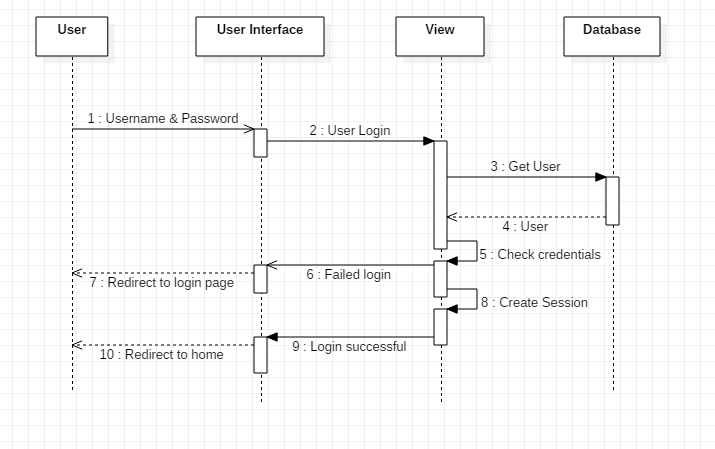
\includegraphics[width=1\columnwidth]{Figures/sequence.png}
\caption{Authentication sequence diagram}
\end{figure}
\textbf{Typical scenario:}\\
- The platform shows a login page.\\
- A user fills in his username and password.\\
- The platform checks the credentials from the database.\\
- The platform creates a session and redirects the user to home page.\\

\subsubsection{Analysis sequence diagram}
An authenticated user will be able to go through the analysis. The analysis sequence diagram that is shown in Figure II.5, is going to be a general overview of how the analysis process from all types of evidence (memory, network, disk).
\begin{figure}[H]
\centering
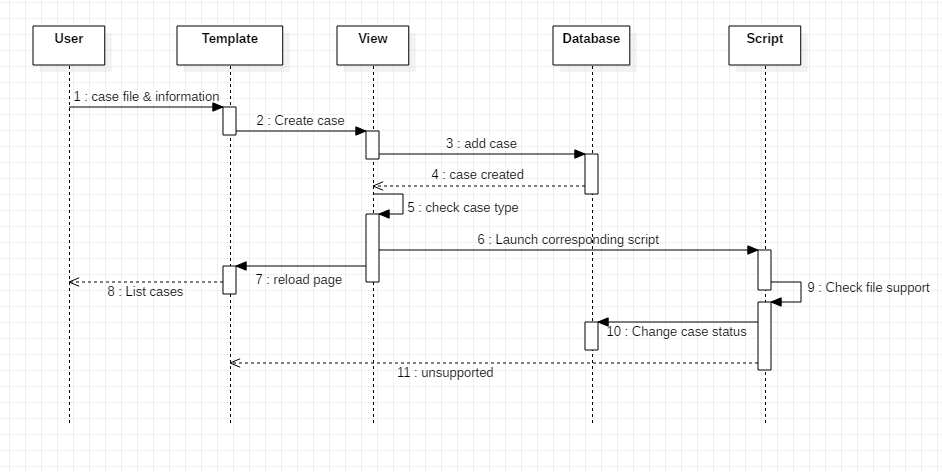
\includegraphics[width=1\columnwidth]{Figures/sequence1.png}
\caption{General analysis sequence diagram}
\end{figure}

Following the previous diagram, the launched script depends on the type of forensic analysis to be run. The system will take care of the analysis using the relative script and output data into the database simultaneously.



\addcontentsline{toc}{section}{Conclusion}
\section*{Conclusion}
Throughout this chapter, we presented and analysed our platform's requirements. We identified the functional and non-functional specifications, then presented the use case and sequence UML diagrams.\\
This chapter paves the way for the next one, in which we will present the implementation of our platform, following the previous analysis.

%%%%% Chapter three
\renewcommand\thechapter{\Roman{chapter}}
\chapter{Realization and Implementation}
\newpage
\addcontentsline{toc}{section}{Introduction}

\section*{Introduction}
In this chapter we will present the implementation and realization of our platform.\\We begin by presenting the application's architecture. Then we present the software and hardware environment along with the tools used. Afterwards, we will give an overview of the modules that are working in the platform to do the analysis and security measures implemented following earlier specifications.


\section{Application’s Architecture}
In this section we will introduce the architecture we followed for developing and deploying the platform.
\subsection{General Architecture}
For better usability, modifiability, stability, and security, we chose to follow a simple architecture that consists of a client and a server.\\With the server being centralized, the client server architecture, seen in Figure III.1, allows the application to manage resources common to all users, allow the use of the application without depending on the user's own computer specifications, which is an important factor considering the processing of E-evidence, and also presents more secure infrastructure since administrators can control consultants data access on server with relatively little effort, so the system can be upgraded simultaneously for all users in no time.\\With the user accessing through the client, which is any web browser, instructions are sent as HTTP requests to the server, then the server processes the data using pre-made scripts and send a reply.
\begin{figure}[H]
\centering
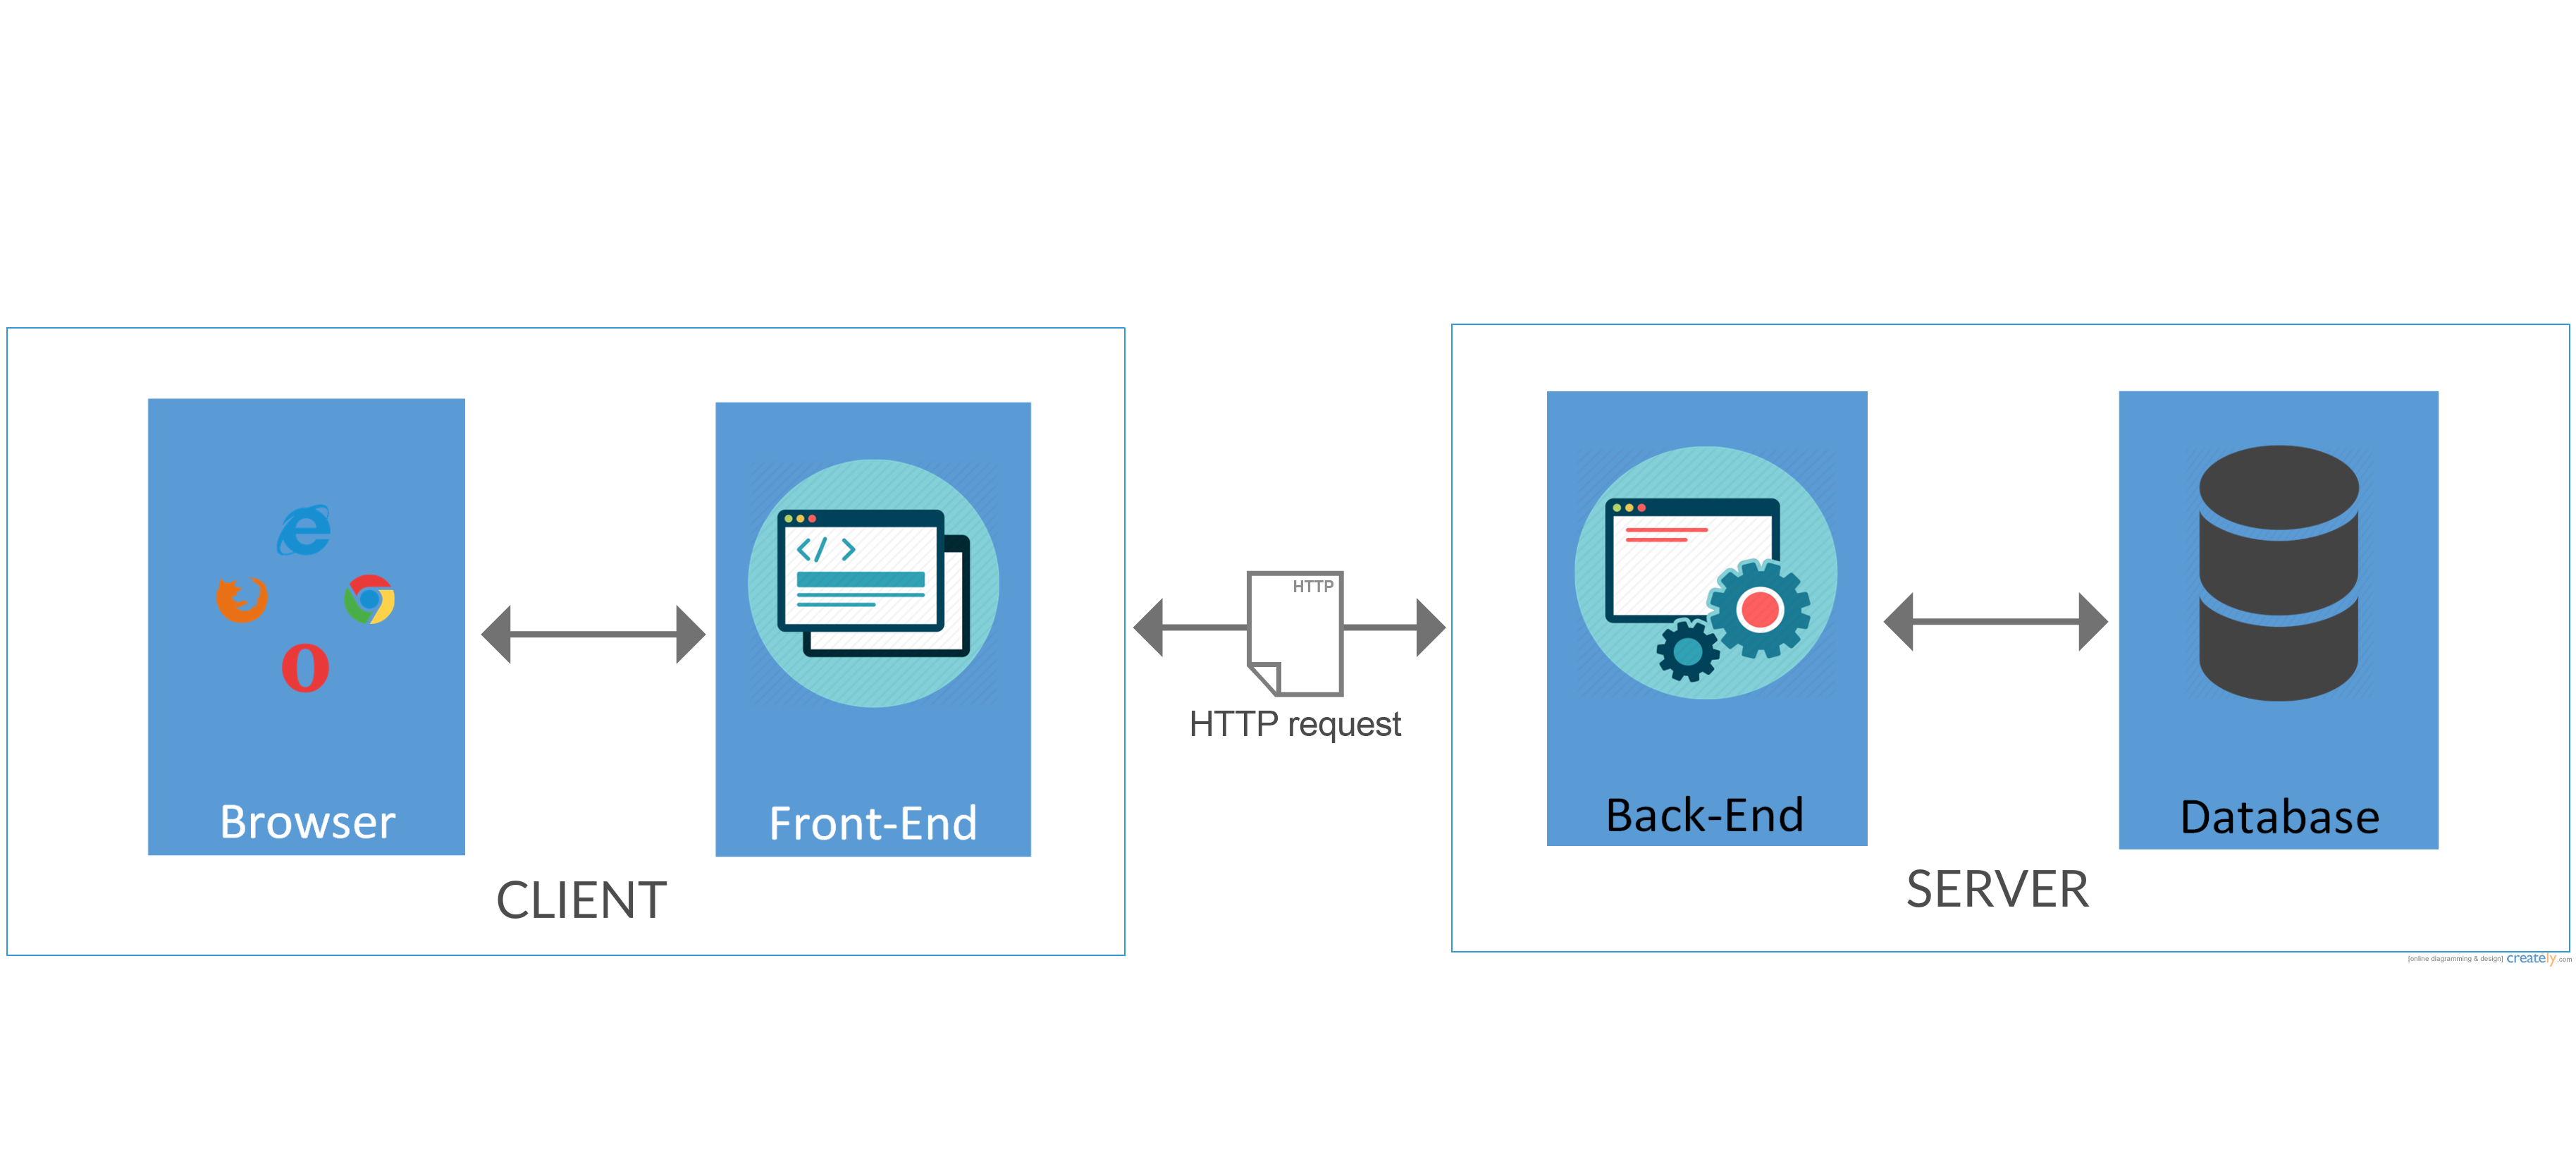
\includegraphics[width=1\columnwidth]{Figures/genarchitecture.png}
\caption{General architecture of the application}
\end{figure}

\subsection{Server and Back-End Architecture}
The application's back-end architecture uses Django views as controller and executor of instructions received from the client. The view does the back-end work related to the interface by accessing the database for requesting data to be shown on the platform, or sending data inserted by the users.\\As for the analysis, it is done by pre-made python scripts for each forensic analysis type. Each type has it's own modules implemented and requested by a relative script which is requested by the view and connects to the database for accessing case data or saving analysis reports. The Figure III.2 presents an overview of the connections between the Back-End server components:
\begin{figure}[H]
\centering
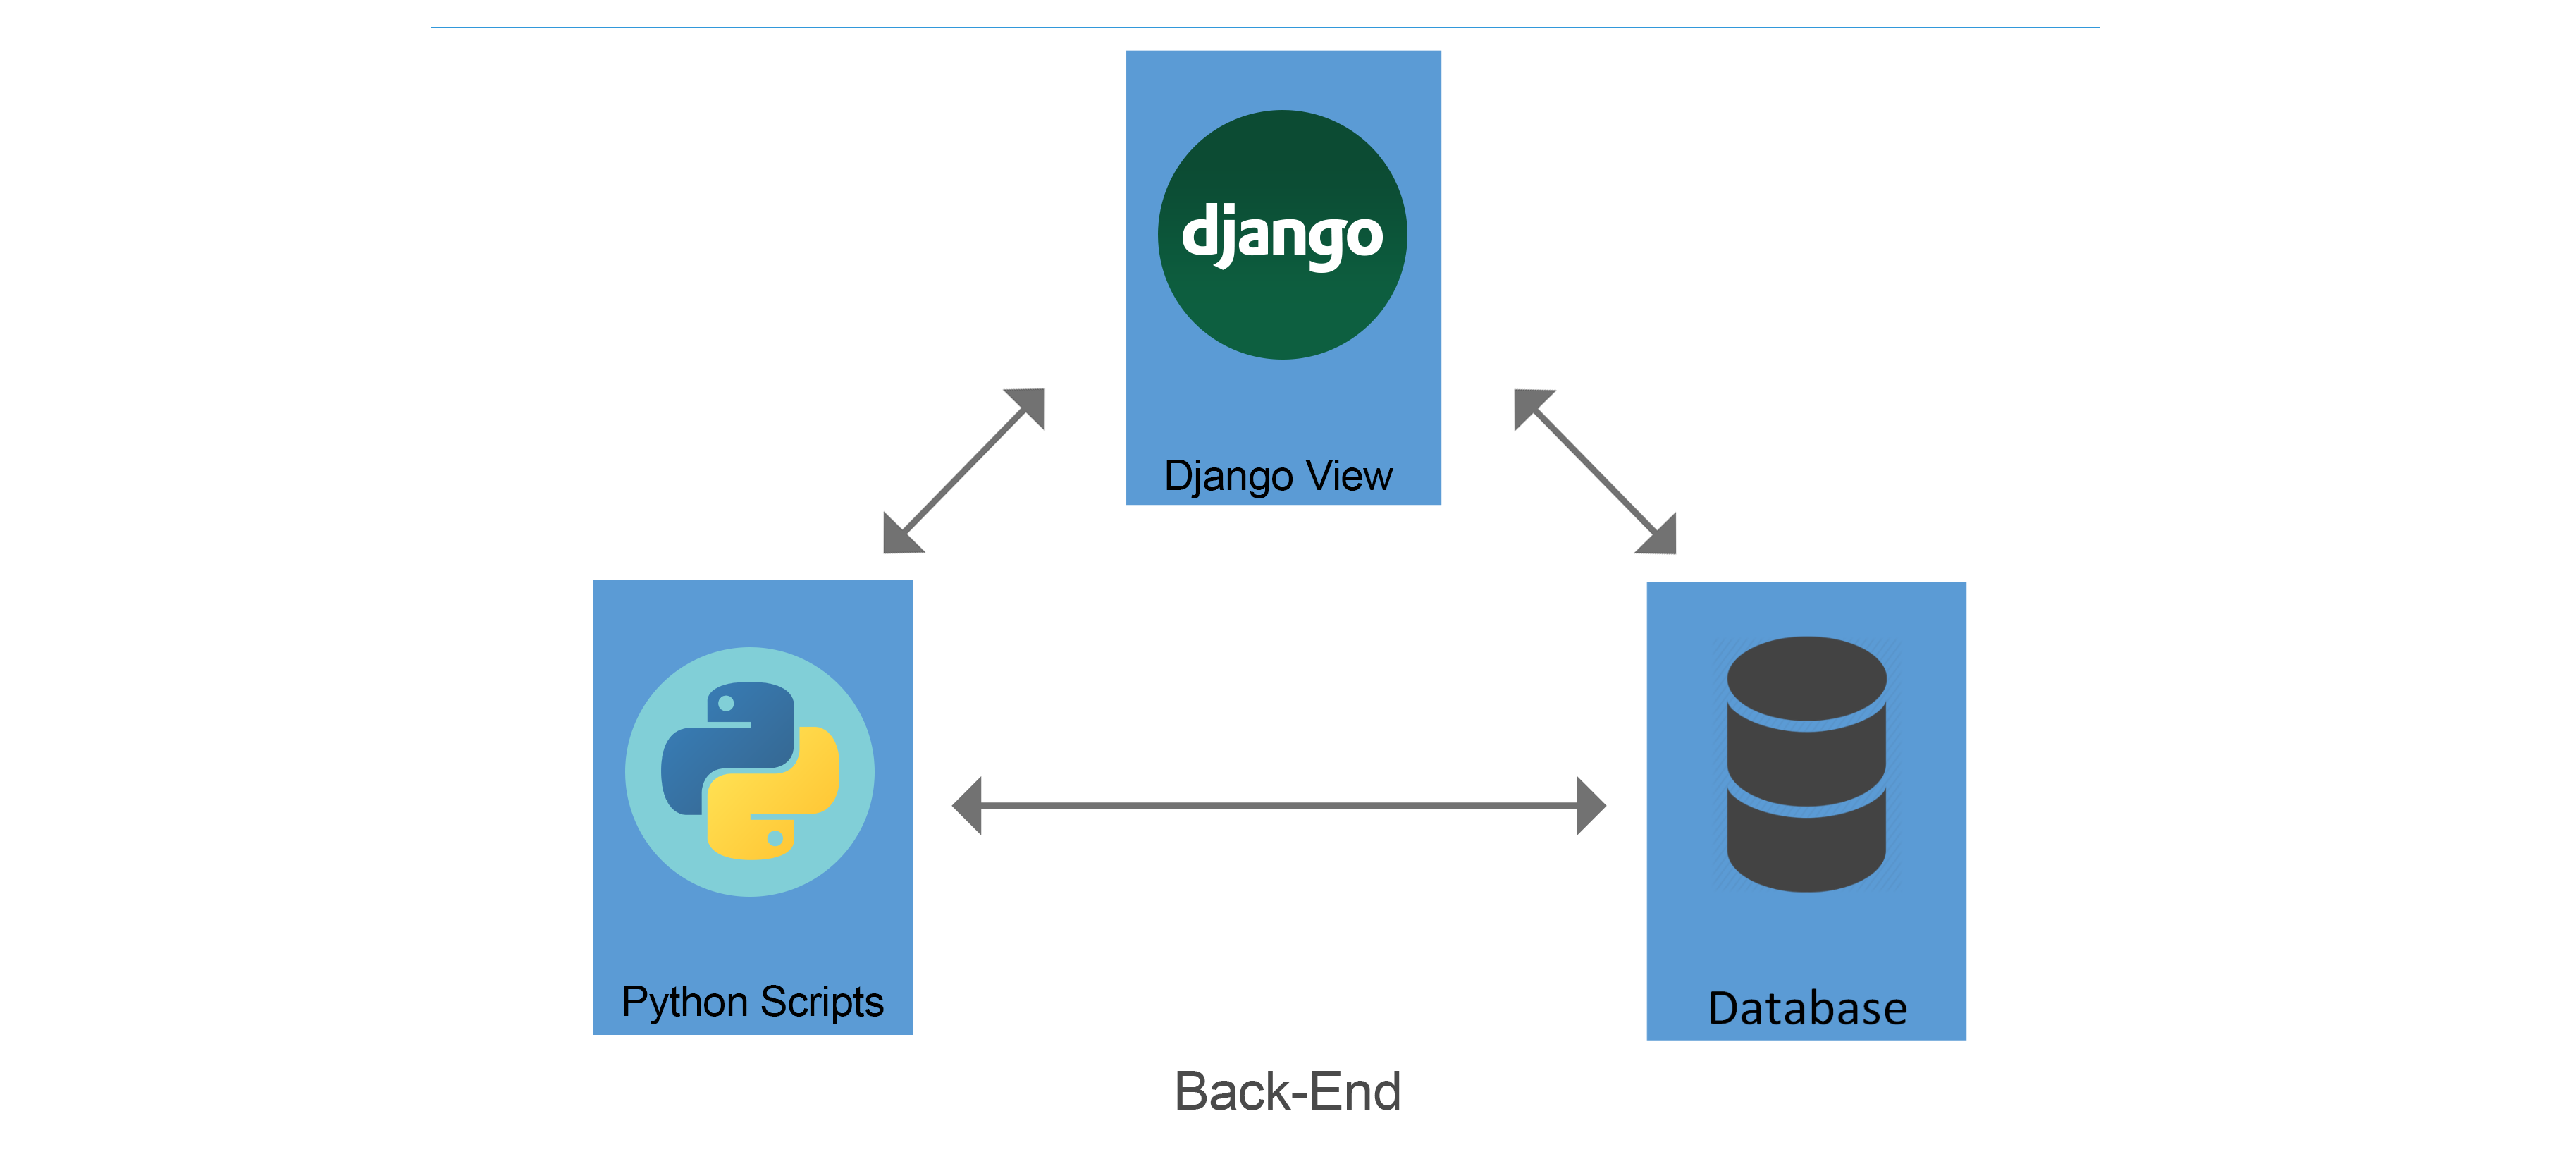
\includegraphics[width=1\columnwidth]{Figures/backarchitecture.png}
\caption{Back-End architecture}
\end{figure}
The application will Preserve the evidence, Identify it, Process it, Analyse and Interpret the analysis, and lastly Present the findings as clear as possible. The forensic analysis types that we included in the platform are the following:
\begin{itemize}
    \item Memory analysis
    \item Network analysis
    \item Disk analysis
\end{itemize}


\section{Software and hardware environment}
We will present the various technologies and tools that we have used and implemented over the platform.
\subsection{Hardware environment}
The process of analysing digital evidence such as memory and disk requires high-end specifications for rapidity and efficiency. So, during most of the project phases, we used a machine that had the specifications presented bellow.\\
\textbf{Laptop:}
\begin{itemize}
    \item \textbf{CPU:} Intel Core i7 6700HQ @ 2.60GHz
    \item \textbf{GPU:} NVIDIA GeForce GTX 960M 4GB
    \item \textbf{RAM:} 16GB SDRAM DDR3
    \item \textbf{Disk:} SSD 120GB / HDD 1TB
    \item \textbf{OS:} Parrot OS
\end{itemize}
For the testing phase, we used virtual machines to separate our production and testing environments. The VMs will not be included in the platform architecture since they were used to replicate a real use case.
\begin{itemize}
    \item \textbf{Hypervisor:} Virtualbox 6.0
    \item \textbf{Virtual machine 1:} 
        \begin{itemize}
            \item CPU: 4
            \item RAM: 4GB
            \item Disk: 80GB
            \item OS: Kali Linux 2019.1
        \end{itemize}
    \item \textbf{Virtual machine 2:} 
        \begin{itemize}
            \item CPU: 1
            \item RAM: 2GB
            \item Disk: 32GB
            \item OS: Windows 7 Pro 64bit
        \end{itemize}
\end{itemize}

\subsection{Software environment and technologies}
In this section, we are going to present the tools and software we used in the development of the platform, and justify each of these choices.
\subsubsection{IDE}
Using and IDE provides comprehensive facilities for software development like integrated tools and add-ons that make the development process clearer and more efficient. Sublime text, Visual Studio, and PyCharm are some of the best IDEs favored all over the world. Our choice was PyCharm\cite{pycharm} which is dedicated for Python, available in both paid and free version while introducing amazing advantages and work on Windows, Mac OS X, and Linux platforms. This IDE supports Python development directly and is therefore well suited for Django developing. The paid version also supports Django development out of the box. It also contains powerful tools for debugging, an integrated terminal, and also an integrated python interactive shell. This makes it quite easy to manage a project with a big infrastructure that also requires moving through lots of windows.

\subsubsection{Hypervisor}
A hypervisor allows the creation of multiple virtual machines on a single computer. This gives us an oppurtunity to create a testing environment that is easy to use, reset, and maintain. In comparison to VMware ESXi and Hyper-V, VirtualBox\cite{virtualbox} was the best solution to choose between them. It allows creating virtual machines, each with an operating system, on a running Machine inside a host operating system, making it a type 2 hypervisor. The architecture used by virtualbox is more useful and appropriate in our case. We also don't want to sacrifice our host OS, and are using the virtual machines for creating test cases. Another advantage is that virtualbox uses easier and more compatible file types for the snapshots and disk storage, which we will use for testing our platform.

\subsubsection{Front-end framework}
Django is a high-level Python open-source web application development framework that provides a clean and pragmatic design to database-driven websites. It has a good set of libraries and underscores effectiveness, allows less need for coding and reusability, and also various secure measures. It is also based on the Model-Template-View (MTV) architecture which is close to the MVC architecture. It also comes with a ready administration interface that allows administrators to easily add, edit, and remove users, models and consult recent changes by users in the website's database. Looking for long-term support for the platform, Django is also perfect for supporting Python3 since Python2 is to be out of support starting 2020.


\subsubsection{Back-end}
For the back-end, we need a scripting language that is well supported in information security. There are multiple choices including Ruby, Python, and Go. Our choice falls on Python for various reasons including preference, the tools we will implement also use it, and the libraries it provides prove very useful for our platform.
Python is an object-oriented, high-level programming language built for general purpose programming with integrated dynamic semantics for scripting, web and app development, and recently popular in data science. The large libraries and community support for Python keeps it one of the best, easiest, and favorite programming languages. Python is well suited for usage in the cyber security field since it has a clean, dynamic and logical syntax code and modular design. Also the need for programming in cyber security is high, so python being an interpreted scripting language with an immersive library, not to mention it's growth to the top lists, makes it the obvious choice. One of the libraries we used to connect the database to the front-end was the following:
\begin{itemize}
    \item Djongo
    Django doesn't usually come supported to MongoDB since the latter is a NoSQL database. Using Djongo we can make it possible to use Django with MongoDB without changing the Django ORM (Object-Relational Mapper). Djongo serves as a SQL to MongoDB query compiler. It basically translates a SQL query into a MongoDB query document.
\end{itemize}

\subsubsection{Database management}
The design for non-SQL databases is relatively simple, speed tolerant, and more flexible. MongoDB is a document-oriented database classified as a NoSQL database, meaning it doesn't follow the tabular relations for storage and retrieval of data like other SQL or relational databases. MongoDB uses JSON-like documents, which is one of it's powerful traits since JSON is replacing XML as a standard data interchanging language. More and more scripts, tools, and APIs now output results as JSON data, which makes it perfect for us to use it as our back-end database.


\subsubsection{Open-source used tools}
We implemented well-known and used open source tools in the platform which helps us get accurate results and edit the code per our needs. The reason for choosing these tools is because they've proven their usefulness regarding the modules we are implementing. We will now list the tools we used in our solution:
\begin{enumerate}
    \item \textsc{Volatility }
         is an open-source forensics framework for incident response and malware analysis on memory analysis implemented in python. It supports analysing memory of multiple operating systems like Linux, Windows, Mac, and Android, and can analyse different volatile memory samples such as raw dumps, crash dumps, and virtual machines memory dumps.
    \item \textsc{CapTipper }
         is a python tool providing a way to analyze, explore and revive HTTP malicious traffic. It mainly recreates a web server like the one in the traffic from the provided pcap file and allows inspection. The tool also contains an interactive console for deeper analysis of traffic and trasfered objects.
    \item \textsc{Tcpxract }
         is a tool written in C language for carving files from pcap files by analyzing data streams. It tries to identify and extract the files in the sessions using file file signatures and started at first using the same technique as Foremost for recovery.
    \item \textsc{Foremost }
         is a tool used for data carving from files, and was originally created for law enforcement uses. It searches for files using built-in types signatures, headers, and data structure. Foremost work mainly with disk images created by dd, Encase, and other tools. It can recover deleted files from a drive that hasn't been override by zeros.
\end{enumerate}


\section{Application’s Implementation}
This section contains the technical implementation of the platform and the modules in each forensic analysis type. Then we will introduce some of the implemented security measures. 
\subsection{Memory Forensics}
For the memory forensics, the script is provided with a case object to analyse. The script for this subsystem then gets the evidence file provided and starting running various modules that consist mostly of Volatility plugins and in which some are custom made.\\
The volatility plugins included are saved in the appropriate directory relative to the tool which is included with our platform by default. In the case of these plugins, we'll loop through a pre-made list, which takes place in a settings file included in the script, while selecting a certain extraction file type and location for each one as Figure III.3 shows:
\begin{figure}[H]
\centering
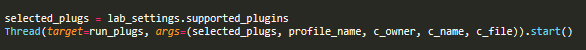
\includegraphics[width=1\columnwidth]{Figures/1_.png}
\caption{Volatility plugins call}
\end{figure}
The Figure III.4 shows the different arguments passed to Volatility when calling certain plugins due to their unique requirements.
\begin{figure}[H]
\centering
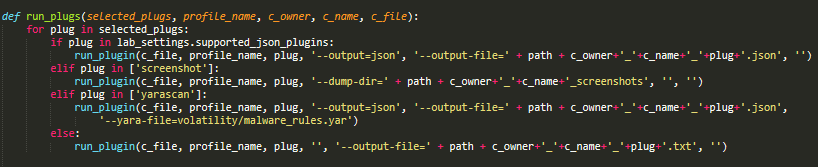
\includegraphics[width=1\columnwidth]{Figures/2_.png}
\caption{Looping through and running Volatility plugins}
\end{figure}
We will now talk more about the modules individually. The modules as we said include and are not limited to Volatility plugins, customs modules, and APIs. We will present in the following subsections what each of the modules is doing.

\subsubsection{Keylogger Static Detection}
Keyloggers can be detected and identified as malicious applications for recording the user's activity such as keystrokes, screenshots, and network data. Keyloggers will need certain permissions that are known to be found on Spyware so it will most likely be detected in a dynamic analysis, but since a keylogger has high impact, we chose to develop a module which detects known Keyloggers for easier interaction. We will provide a list of well known keylogger process names in this case, and we'll be back for more advanced malicious application detection in later modules. We can see the combination between the process list and the keylogger list in Figure III.5 bellow.
\begin{figure}[H]
\centering
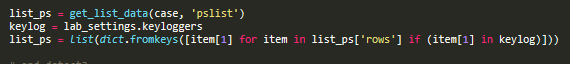
\includegraphics[width=0.8\columnwidth]{Figures/keyloggers.png}
\caption{Keylogger static detection code}
\end{figure}

\subsubsection{Malicious IP detection}
Based on the list of connections that we can extract using the Volatility 'netscan' plugin, we will remove local IP addresses and search the remaining ones on the web for previous violations or malicious traffic. This process only supports IPv4 for now.\\
For this module we use the API provided by AbuseIPDB\cite{abuseip} which will give us the number of reports registered against a certain IP and based on that, it calculates a trust level. We will be saving and outputting IPs with a relatively low trust level. The Figure III.6 explains how we loop through the IPs extracted from another module and scan each one of them as desribed above.
\begin{figure}[H]
\centering
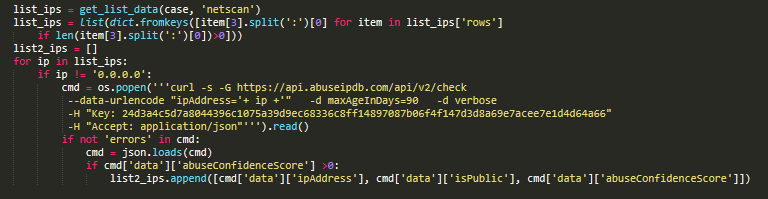
\includegraphics[width=0.8\columnwidth]{Figures/ips.png}
\caption{Malicious IP detection}
\end{figure}

\subsubsection{Process Extraction}
\begin{enumerate}[label=(\alph*)]
    \item \textbf{Process List}\\
    For listing the running processes on the system, we will use the 'pslist' plugin. We call volatility and simply ask for a process list. This will output the process name, pid, ppid, launch time, and other details.\\
    The module walk through doubly-linked list pointed to by PsActiveProcessHead to extract these process information as we see in Figure III.7, the plugin looks for all the processes.\\
    \begin{figure}[H]
    \centering
    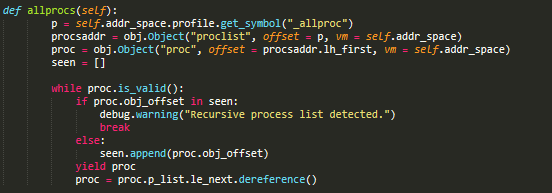
\includegraphics[width=0.8\columnwidth]{Figures/pslist.png}
    \caption{Process list core extraction from memory}
    \end{figure}
    After listing all processes, we can extract the process executable file from memory by supplying the offset to the 'procdump' plugin. And of course this is done automatically. Figure III.8 contains the code we wrote to combine the previous extracted info, primarily the process pid, with the 'procdump' plugin to extract the executable.
    \begin{figure}[H]
    \centering
    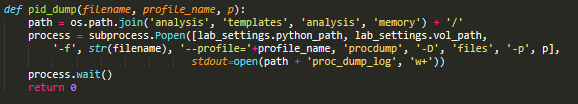
\includegraphics[width=0.8\columnwidth]{Figures/psdump.png}
    \caption{Process dumping function}
    \end{figure}
    \item \textbf{Process Tree}\\
    The process list extracted by the previous module is more accurate than this one, but also not enough for following the root of a process. For that reason comes a need to scan the process explorer to output a tree representing the processes each under it's parent.\\
    This module uses Volatility's 'pstree' plugin, which simulates the execution of the command called with the same name under Linux systems. The latter being a visual representation of the process list while the root of the tree is mainly init. The process for extraction starts by finding the root then the next node and the nodes following it. The next figure, Figure III.9, shows the first step of the process.
    \begin{figure}[H]
    \centering
    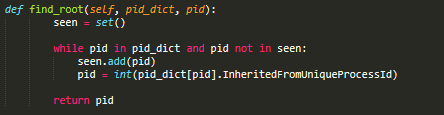
\includegraphics[width=0.8\columnwidth]{Figures/pstree.png}
    \caption{Process tree root location}
    \end{figure}
\end{enumerate}

\subsubsection{Auto-run Programs Scan}
This module uses a volatility custom-made by Tomchop\cite{tomchop} and it allows finding Auto-Start Extensibility Points or Persistence Points which is a recurring task of any investigation to locate potential software that is doubted as malware.\\
Modern Malware and especially Trojans that run in memory need to be started every time a computer is powered-up, that is why we need to analyse autorun programs.\\
This module basically automates the tasks you would need to identify where malware or a certain process is persisting from. Depending on the system, after all the auto-start locations are found, they are matched with running processes to finally output a list. The full code of the plugin can be found on it's repository\cite{autorun_repo}. The Figure III.10 contains a portion of the locations included in the search:
\begin{figure}[H]
\centering
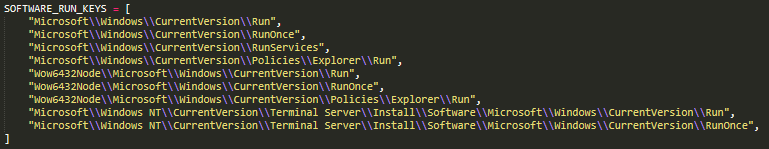
\includegraphics[width=0.8\columnwidth]{Figures/autoruns.png}
\caption{List from the lists of location to search}
\end{figure}

\subsubsection{Network Scan}
To get a list of network connections made on a computer out of a memory dump, we will use Volatility's 'netscan' plugin. This plugin was introduced around 2011 and gives an overview of the active and inactive connections on a computer.\\
Without getting into physical memory or the plugin's details, this module find TCP/UDP endpoints, which establishes connections, and TCP/UDP listeners, which listens for connection on a certain port. It also has the ability to distinguish and regroup connection based on the IP version used (IPv4 / IPv6) and local/remote IPs.\\
The plugin is good to give us an overview to establish a timeline based on other data that it extracts like the time when the socket was bound or the connection was established, and it's current state.
%image

\subsubsection{Physical Files Scan}
Using the 'filescan' plugin from Volatility, we can scan the memory dump for file objects, which will find a file by the hooks and pointers defined when processes use it. We can then extract these files from memory or follow the pointers to the processes and go deep into injected DLLs.\\
Technically talking, the process is used for locating kernel object allocations using pool tag scanning. The module shows permissions affected to the files, physical offset, number of pointers and handles to the file object.\\
We then try to extract the file, on demand, using the 'dumpfiles' plugin, as seen in Figure III.11. This can be done by using the already-found offset of the object. Some files can't be extracted for various reasons, one of them being that the file is just a Symbolic link to another file meaning it's not the physical file having the real contents.
\begin{figure}[H]
\centering
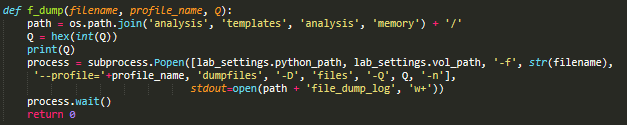
\includegraphics[width=0.8\columnwidth]{Figures/filedump.png}
\caption{File dumping function}
\end{figure}

\subsubsection{Browser Data Extraction}
Extracting Data from web browsers is important for following the user's footsteps and understanding it. The data can be his browse history, download history, cookies, and more. Since most of these data can be found in disk analysis and is not only relevant to memory, we'll be extracting only browsing history.\\
Each browser stores the user's data in it's specific way. This module will allow us to go through top used web browsers on windows to extract it's history from memory.
\begin{enumerate}[label=(\alph*)]
    \item \textbf{Internet Explorer history}\\
    For Internet Explorer the plugin builds a list of tags based on the selected command-line options and associate the tags with our \_URL\_RECORD and \_REDR\_RECORD structures.
    \item \textbf{Google Chrome history}\\
    Google Chrome saves all the data in an SQLite database encrypted using the user's password, and since we're working on the memory itself, we get unencrypted data. Then, the module extracts records from the Chrome urls table in the database file. The plugin is named 'chromehistory' and is created by Superponible\cite{superponible}.
    \item \textbf{Mozilla Firefox history}\\
    Firefox, like Chrome uses it's own database and makes a profile folder in a known location. The 'firefoxhistory' plugin, also created by Superponible, extracts records from the Firefox moz\_places table in the places.sqlite SQLite database file.
\end{enumerate}
%image for iehistory only

\subsubsection{Command Line Detection}
\begin{enumerate}[label=(\alph*)]
    \item \textbf{Command history}\\
    The 'cmdscan' plugin from Volatility is used here to search the memory of csrss.exe and conhost.exe on relative Windows versions for commands that attackers or users may have entered through a console. This module finds structures known as COMMAND\_HISTORY by trying to look for the known constant value MaxHistory (usually set to 50) and then applying sanity checks.
    %image
    \item \textbf{Process commands}\\
    This module uses the 'cmdline' plugin to detect process parameters and arguments and extract the complete command line used to start the process from background CLI in the first place. The plugin generates the command line from the data acquired by the DLL files.
    %image
\end{enumerate}


\subsubsection{Graphical User Interface Scan}
This module draws frames of the GUI from the memory based on opened windows. It is far from a real screenshot but shows outlines, windows names, and possibly underlying windows. It basically enumerates windows for each desktop in their Z-Order. An example of the output pictures is included in Figure III.12:
\begin{figure}[H]
\centering
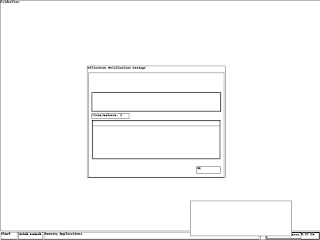
\includegraphics[width=0.8\columnwidth]{Figures/vol_screen.png}
\caption{Memory screenshot output example}
\end{figure}

\subsubsection{Malware Analysis}
For detecting malware, we use some simple techniques that try to search for malicious-known data inside a process to identify it as a malware, or locate injected DLLs, or have certain permissions like network access or system files write.
\begin{enumerate}[label=(\alph*)]
    \item \textbf{Malfind}\\
     Based on characteristics such as VAD tag (virtual address descriptor) and page permissions, The 'malfind' plugin tries to locate injected shellcode or DLLs that basic methods can't find. An example of injection that it can't detect are the ones initiated using CreateRemoteThread.
    \item \textbf{YARA scan}\\
     The purpose of YARA is to identify and classify malware samples. YARA rules provide a way to create descriptions for malware families based on textual or binary patterns that the determine the logic behind the malware. This makes YARA as the main way that could detect malware without reversing an executable.\\
     Using these rules, the 'yarascan' plugin, provided with a custom file containing various rules of malware and malicious applications, can detect a malicious process when comparing it's data and behaviour to a certain rule.
     \begin{figure}[H]
     \centering
     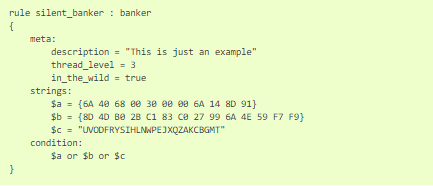
\includegraphics[width=0.8\columnwidth]{Figures/yara.png}
     \caption{YARA rule description example}
     \end{figure}
     The rule, in Figure III.13 above, is telling YARA that any file containing one of the three strings must be reported as silent\_banker. This is just a simple example, more complex and powerful rules can be created by using wild-cards, case-insensitive strings, regular expressions, special operators and many other features that you’ll find explained in this documentation\cite{yara_doc}.
\end{enumerate}


\subsubsection{User Password Extraction}
\begin{enumerate}[label=(\alph*)]
    \item \textbf{Hashdump}\\
    The 'hashdump' plugin accesses the SAM and SYSTEM hives on Windows registry and outputs cached user credentials which can possibly be cracked later.
    \item \textbf{Mimikatz}\\
    Mimikatz was first a tool that extracts plain text passwords from Windows. The module introduced as a Volatility plugin works the same as in a live machine by analysing the LSASS process, finds the encryption keys and IV (initialization vector) and decrypts the hashed passwords in the LSA Secrets registry. The plugin contains decryption functions relative to most windows versions. We can see the function relative to the 64 bit version of Windows 7 in Figure III.14.
    \begin{figure}[H]
    \centering
    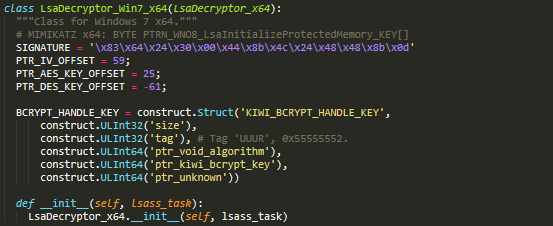
\includegraphics[width=0.8\columnwidth]{Figures/mimikatz.png}
    \caption{Mimikatz plugin - LSADecryptor for Win7 64bit}
    \end{figure}
\end{enumerate}


\subsection{Network Forensics}
\subsubsection{HTTP malicious traffic detection}
Drive-by attacks are when a victim is redirected through multiple websites until he lands on a malicious server that hosts an exploit kit. The exploit kit scans the victim's computer and installs or executes a malware, such as a flash script, javascript, or an executable on the computer to get access. To detect these traffics we used CapTipper\cite{captipper} to analyse our network traffic. The tool launches a web server and replay the pcap file while intercepting the traffic. We then get the output of the first stage analysis which is a summary since the tool also offers an advanced interpreter. We run the script from the directory saved in the settings and save the output to a file to be processed later, as shown on Figure III.15 bellow.
\begin{figure}[H]
\centering
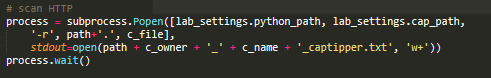
\includegraphics[width=0.8\columnwidth]{Figures/http.png}
\caption{Calling CapTipper from settings}
\end{figure}

\subsubsection{File carving}
Detecting and extracting communicated files on the network is important even if our automated analysis doesn't detect it is malicious at first. So using Tcpxtract, we supply a pcap file and try to carve out files using the list of file signatures that we know. As shown in Figure III.16, we simply provide the file as an argument to the tool.
\begin{figure}[H]
\centering
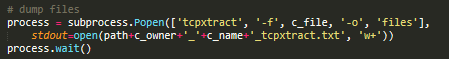
\includegraphics[width=0.8\columnwidth]{Figures/tcpx.png}
\caption{File carving using tcpxtract}
\end{figure}

\subsection{Disk Forensics}
\subsubsection*{File extraction}
Files can be deleted from a drive but unless the space was rewritten to zeros, we can recover the files using Binwalk and Foremost file carving technique that depends on file signatures, footers, and structures. Shown in Figure III.17 is the usage of binwalk in our module. The tool simply needs a disk image and will automatically try to find out files and save them in an output folder.
\begin{figure}[H]
\centering
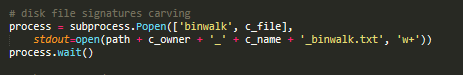
\includegraphics[width=0.8\columnwidth]{Figures/disk.png}
\caption{File extraction using Binwalk}
\end{figure}

\subsection{Secure measures}
\subsubsection{Encrypted traffic}
Normally, data sent between browsers and web servers is in plain text, leaving users vulnerable to eavesdropping. If a malicious party intercepts the data that's being transferred between a client and a web server, they can see and use that information and the user would be vulnerable to MITM attacks.\\
SSL enables secure exchange of information between browsers and the web server, that's why we used an SSL certificate to secure the traffic using HTTPS. Figure III.18 presents the details of our used certificate in the web server.
\begin{figure}[H]
\centering
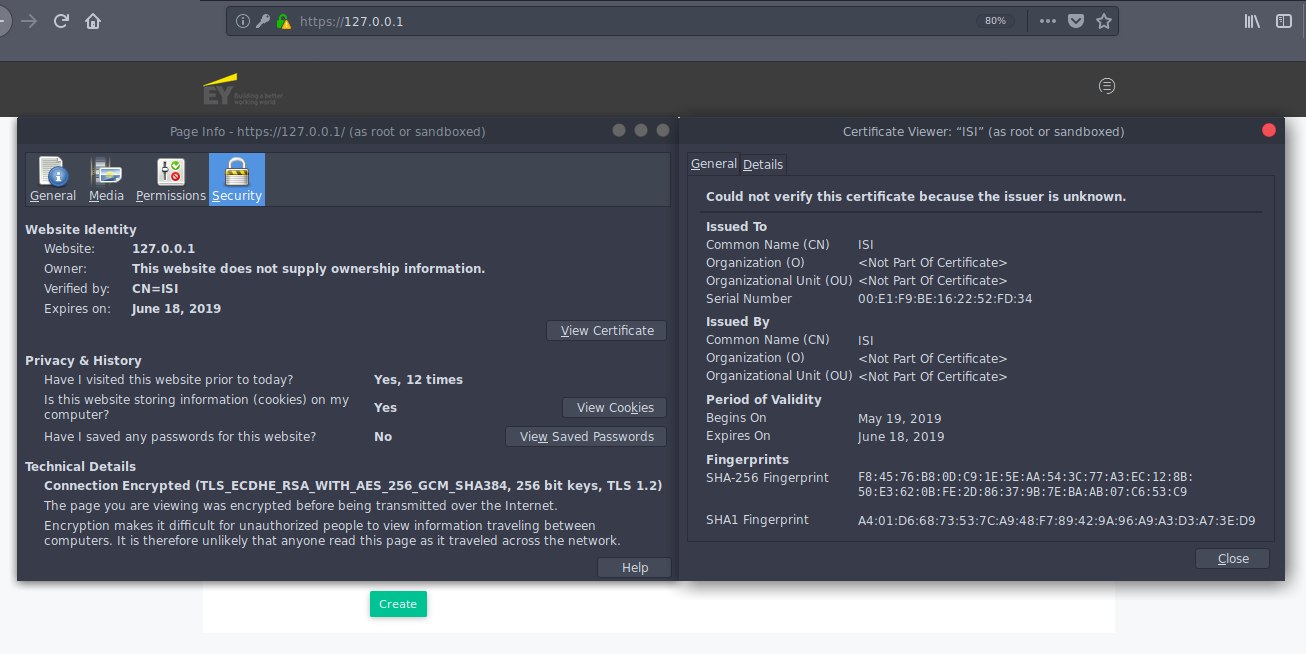
\includegraphics[width=0.8\columnwidth]{Figures/ssl.png}
\caption{SSL certificate details}
\end{figure}
\subsubsection{Authentication}
Django provides a flexible password storage system and uses PBKDF2 with sha256 by default \cite{dj_auth}. The password is stored in the following format:
\begin{verbatim}
    <algorithm>$<iterations>$<salt>$<hash>
\end{verbatim}
The code responsible for generating the password is represented in Figure III.19.
\begin{figure}[H]
\centering
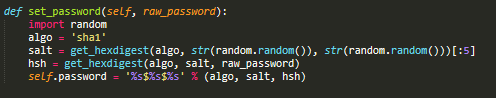
\includegraphics[width=0.8\columnwidth]{Figures/password_storage.png}
\caption{Django password storing mechanism}
\end{figure}

\subsubsection{Cross site request forgery protection}
CSRF attacks allow a malicious user to execute actions using another user's session without the latter’s knowledge or consent.\\
For this reason Django provides us with a built-in tag \{\%csrf\_token\%\} to be used inside action forms on the template side. In Figure III.20, we show a portion of the login page's template, where we used the provided tag inside the authentication form.
\begin{figure}[H]
\centering
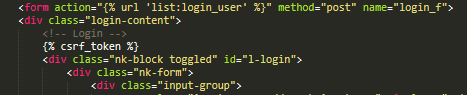
\includegraphics[width=0.8\columnwidth]{Figures/csrf.png}
\caption{CSRF tag in login form}
\end{figure}

\subsubsection{Input filtration for RCE protection}
Using the uploaded evidence files in multiple commands explicitly exposes the back-end server to Remote Code Execution (RCE). This requires either trusting the user's input or filtering it to remove any possible bypass method.\\
As a first step we renamed the uploaded file to something that isn't exposed to the user using the code in Figure III.21. And that was achieved by not exposing the uploads directory to the public too.
\begin{figure}[H]
\centering
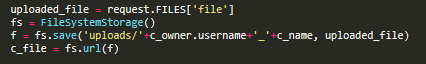
\includegraphics[width=0.8\columnwidth]{Figures/filename.png}
\caption{File naming}
\end{figure}
The second step was to filter the name of the case to avoid a bypass since it's used in the file name and other locations. The filter shown on the code in Figure III.22, is custom-made following various payloads on remote code execution seen on a research\cite{payloadsallthings}.
\begin{figure}[H]
\centering
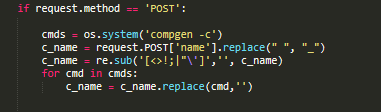
\includegraphics[width=0.8\columnwidth]{Figures/filter.png}
\caption{Case name filtering code}
\end{figure}




\section*{Conclusion}
\addcontentsline{toc}{section}{Conclusion}

Throughout this chapter, we introduced the general architecture of the platform including the front-end and back-end. We then described the environment by specifying the hardware and software used. Finally, we presented our core analysis modules technically, and also the security implementation in place.\\
In the next chapter, we are going to test our platform against a real case scenario while highlighting some of the modules.

%%%%% Chapter four
\renewcommand\thechapter{\Roman{chapter}}
\chapter{Digital Forensics Investigation Case Study}
\newpage
\addcontentsline{toc}{section}{Introduction}
\section*{Introduction}
In this chapter, we are going to test some real case scenarios to show the usage and prove the efficiency of our platform. The scenarios are based on real attacks but any similarity in names is a mere coincidence. We will also try to link some of the investigation's outputs, as our project's purpose is not to automate the whole process and all the phases.\\
In order to simulate real scenarios, we prepared an attacker machine and a victim machine for two cases where we analyse the digital evidence after the extraction.


\section{Authentication and Dashboards}
In this section, we will present the authentication interface and the administration dashboard.\\
Figure IV.1 presents the first page of the platform, which is the authentication page. To access the platform's dashboards and functions, a user must enter his credentials in the login form.
\begin{figure}[H]
\centering
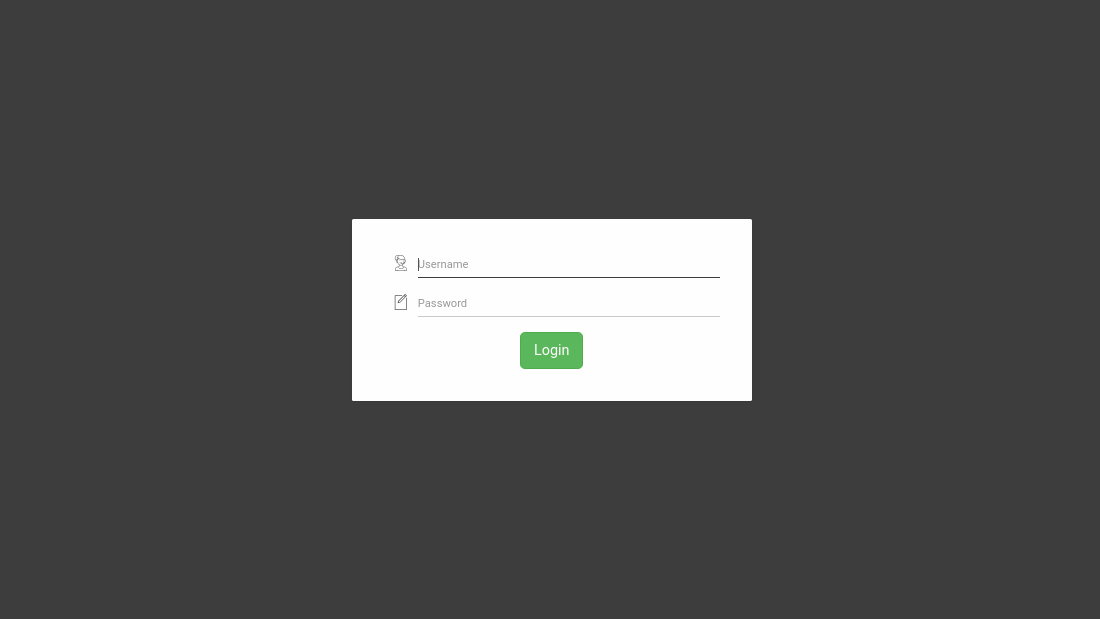
\includegraphics[width=0.9\columnwidth]{Figures/1.png}
\caption{The authentication page}
\end{figure}
Once the user is authenticated, drop-down menu appears on the top-right of the UI containing a logout link, and the administration dashboard's link, while the latter depends on whether the user is an administrator.\\
The first page we land on after a successful authentication, shown in Figure IV.2, allows a consultant to consult a case, remove it, or create a new one.
\begin{figure}[H]
\centering
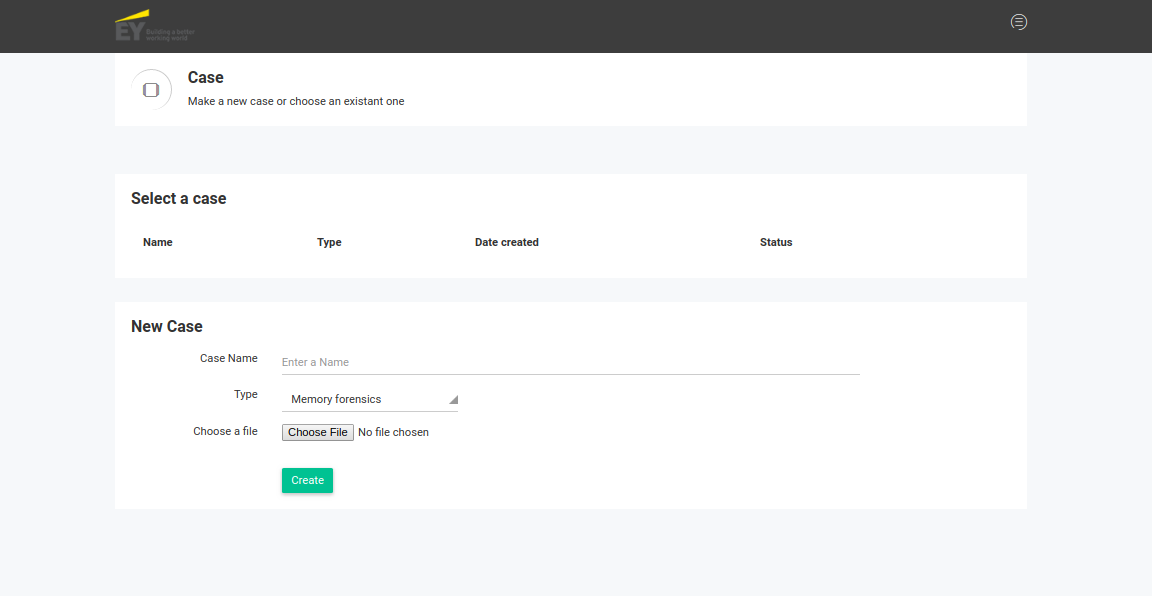
\includegraphics[width=0.9\columnwidth]{Figures/2.png}
\caption{Landing dashboard}
\end{figure}
Figure IV.3 presents the administration dashboard that can be accessed using the link provided in the menu for administrators. 
\begin{figure}[H]
\centering
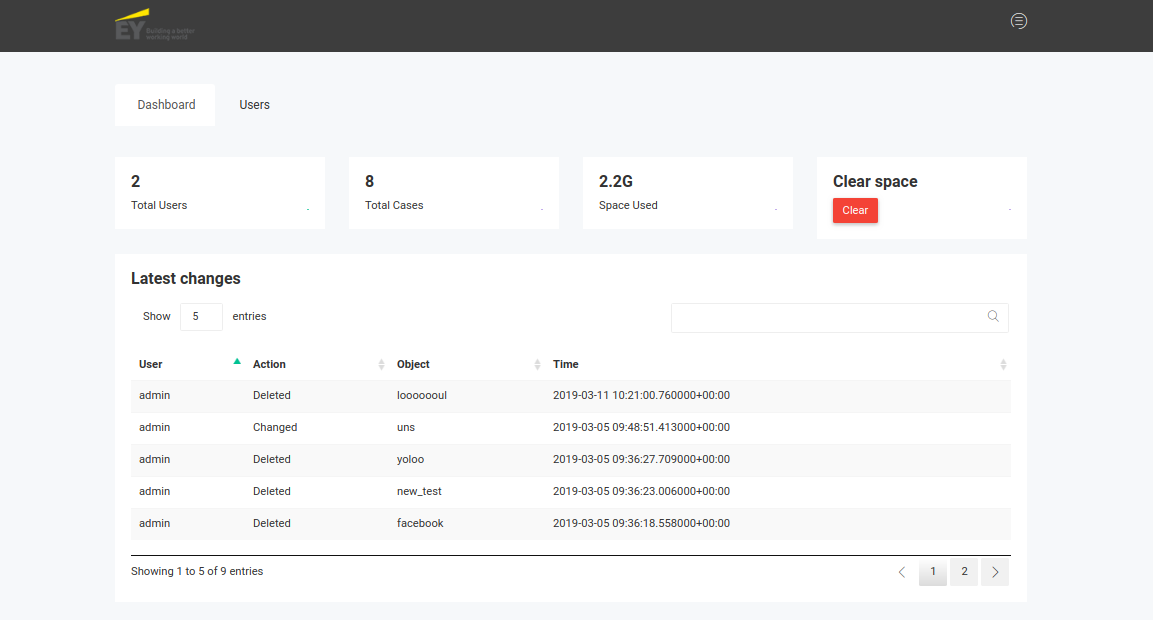
\includegraphics[width=0.9\columnwidth]{Figures/3.png}
\caption{The administration dashboard}
\end{figure}
On this page, the administrator can see some numbers that describe the platform and the database contents along with the latest changes made by users.\\
The administrator can also see the current users, add new ones, and edit the details of an existing user via the Users tab, which is presented in Figure IV.4.
\begin{figure}[H]
\centering
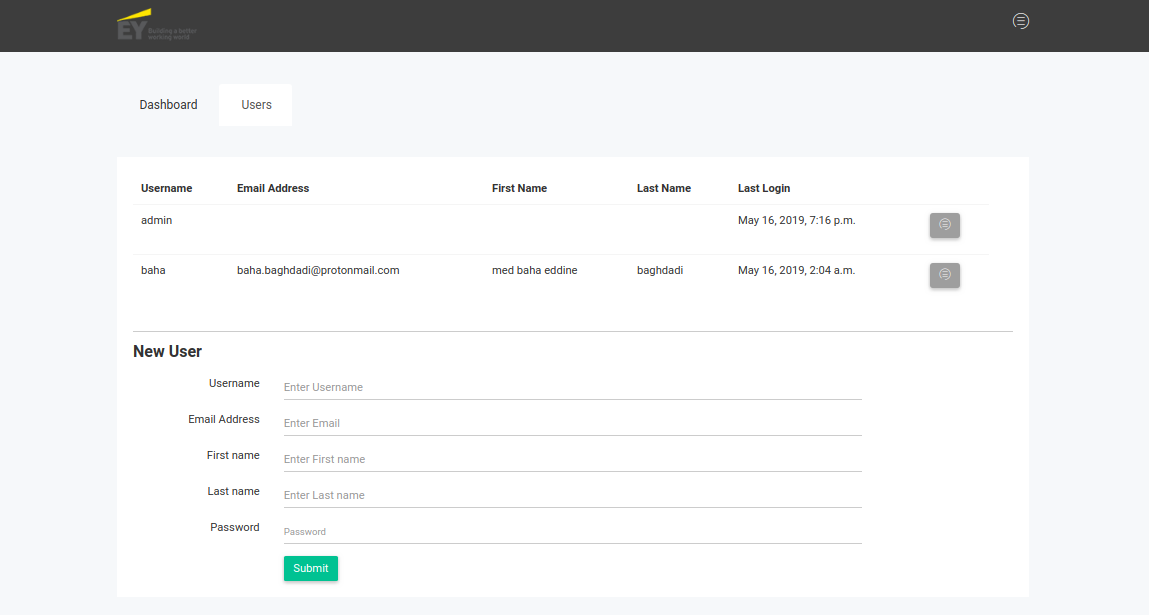
\includegraphics[width=0.9\columnwidth]{Figures/4.png}
\caption{The administration dashboard - Users tab}
\end{figure}

\section{Case Scenario 1: Potentially hacked teacher}
In this section, we will analyse a memory dump from a teacher's laptop that is suspected to have been hacked by a student, who eventually changed his exam score after gaining access.
\subsection{Creating the case}
The first step is extracting the memory dump using a tool like DumpIt\cite{dumpit}, or by simply retrieving the 'vmem' file created by Virtualbox of the victim's machine, in our case. Then, we start by filling out the corresponding form on the platform by supplying the case evidence file, case name, and case type, as is shown in Figure IV.5.
\begin{figure}[H]
\centering
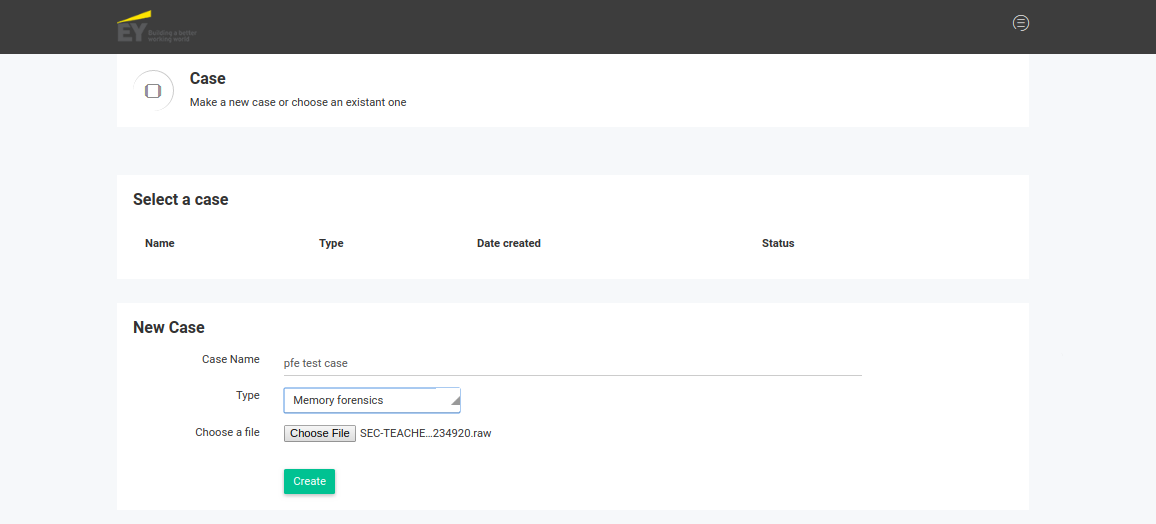
\includegraphics[width=0.9\columnwidth]{Figures/5.png}
\caption{Case creation}
\end{figure}
The evidence file is uploaded to the platform, the user is redirected to the same page, and we can see in Figure IV.6 that the green button labeled 'Pending' is disabled.
\begin{figure}[H]
\centering
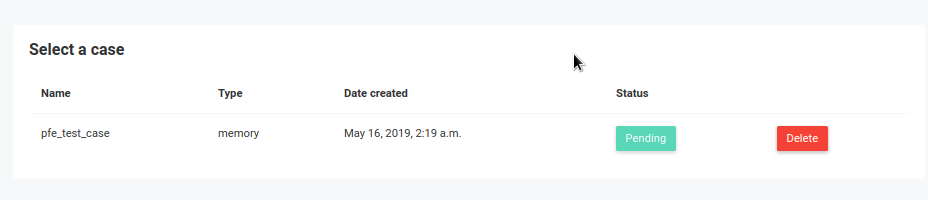
\includegraphics[width=0.9\columnwidth]{Figures/6.png}
\caption{Case file in analysis}
\end{figure}
The page keeps refreshing every 30 seconds to stay updated. After the analysis is done, the green button is enabled and labeled 'Ready', as seen in Figure IV.7
\begin{figure}[H]
\centering
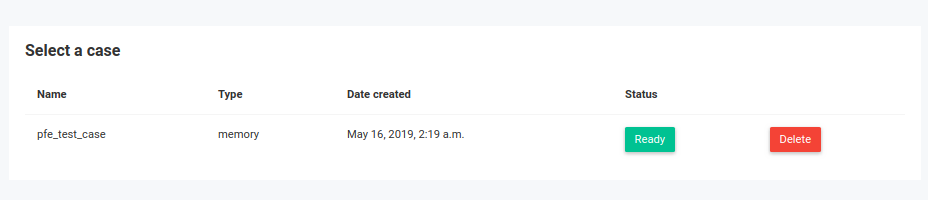
\includegraphics[width=0.9\columnwidth]{Figures/7.png}
\caption{Case analysis completed}
\end{figure}

\subsection{Reviewing the analysis}
The first page for a memory analysis contains general information about the case and the evidence file provided, and detected malicious behaviour like signature-based malware detected, keyloggers, and malicious reported IPs which we talked about in III.3.1.\\
Figure IV.8 presents an overview of how the memory analysis dashboard looks like.
\begin{figure}[H]
\centering
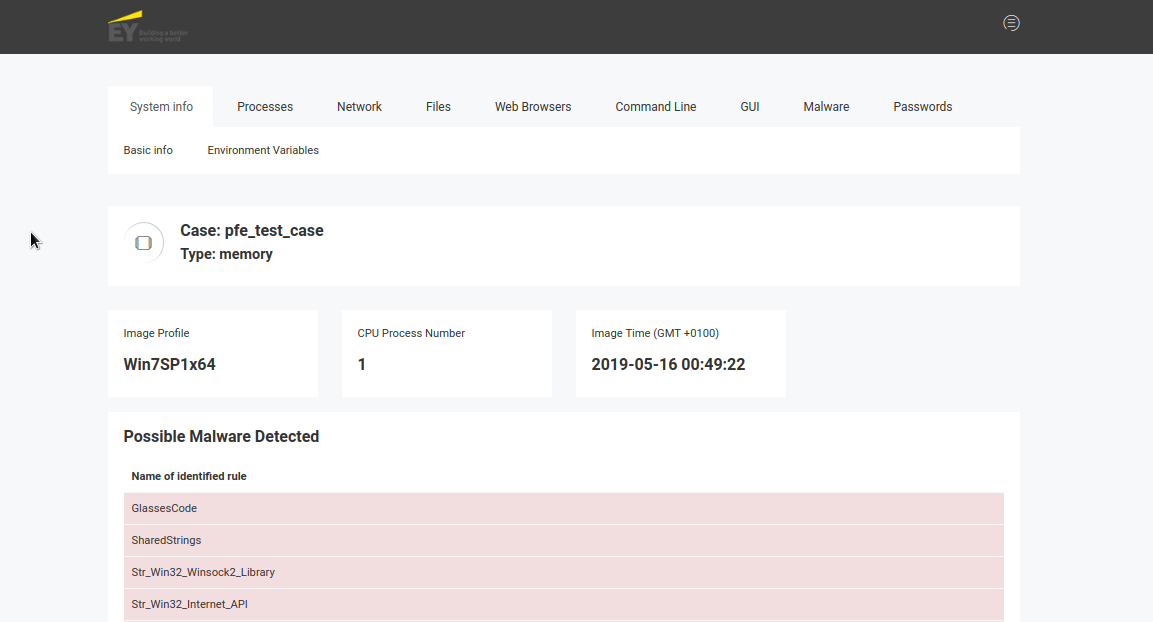
\includegraphics[width=0.9\columnwidth]{Figures/8.png}
\caption{Detected YARA rules in processes}
\end{figure}
Figure IV.9 shows the YARA rules detected in some of the processes.
\begin{figure}[H]
\centering
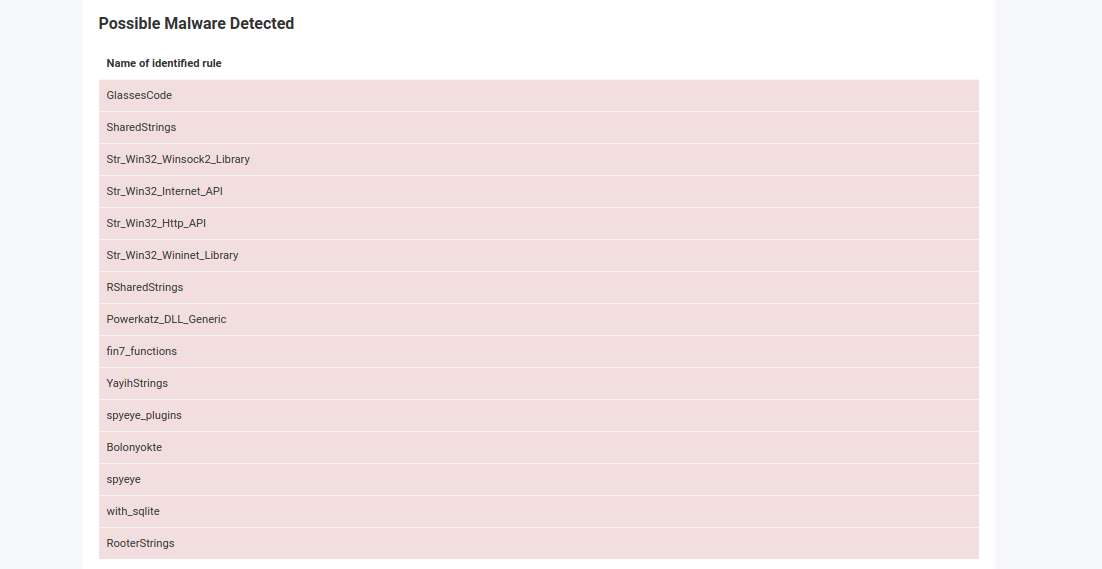
\includegraphics[width=0.9\columnwidth]{Figures/9.png}
\caption{Detected YARA rules in processes}
\end{figure}
Figure IV.10 shows the IP addresses that were reported as malicious and appeared in the computer's network connections.
\begin{figure}[H]
\centering
\includegraphics[width=0.9\columnwidth]{Figures/10.png}
\caption{Detected maliciously reported IP addresses}
\end{figure}
Figure IV.11 shows a detected keylogger process named 'rvlkl.exe', which goes back to a keylogger software named 'Revealer Keylogger'.
\begin{figure}[H]
\centering
\includegraphics[width=0.9\columnwidth]{Figures/11.png}
\caption{Detected Keyloggers}
\end{figure}
\subsubsection{Malware analysis}
Following Figure IV.11, the detected rules based on YARA scan are 15 but that doesn't mean all the rules are of malware. For instance, the 'Str\_Win32\_Internet\_API' rule means that a process is calling the Windows Inet API, which may be sending a reverse shell but no necessarily. The 'fin7\_functions' though, is relevant to a malware attack previously used by a group of hackers called FIN7 that downloads and executes shellcode, which looks interesting enough to look for details in the full YARA analysis, like shown in Figure IV.12.
\begin{figure}[H]
\centering
\includegraphics[width=0.9\columnwidth]{Figures/12.png}
\caption{YARA scan filtered to 'fin7'}
\end{figure}
We can conclude that it points to a process named 'projectx.exe'. Figure IV.13 shows the output we get from YARA scan if we filter on the previously named process, which by the look of it, is using the internet. So, next step is to look at the network connections following this process and scan the process executable.
\begin{figure}[H]
\centering
\includegraphics[width=0.9\columnwidth]{Figures/13.png}
\caption{YARA scan filtered to 'projectx'}
\end{figure}
\subsubsection{Network connections}
The network connections established on the victim's computer looked normal, but as we suspected previously, Figure IV.14 shows that the process 'projectx.exe' was sending a connection to another IP on the same network and using port 4444.
\begin{figure}[H]
\centering
\includegraphics[width=0.9\columnwidth]{Figures/14.png}
\caption{Network connections filtered to 'projectx'}
\end{figure}
\subsubsection{Process analysis}
The process was found to be using the internet to send data, potentially a reverse shell, to another computer. As presented in Figure IV.15, for more analysis we can dump the process executable using the Dump button corresponding to the process, and reverse engineer it and submit it for analysis on VirusTotal.
\begin{figure}[H]
\centering
\includegraphics[width=0.9\columnwidth]{Figures/15.png}
\caption{Process details}
\end{figure}
Figure IV.16 shows the analysis report from VirusTotal that detected the executable as malicious.
\begin{figure}[H]
\centering
\includegraphics[width=0.9\columnwidth]{Figures/16.png}
\caption{VirusTotal analysis report}
\end{figure}
We now need to know how the file was executed. It is possible that the teacher ran the file without detecting it was malicious, or it was executed automatically from a malicious website script, or another way. We can see the background command used to launch the file using the module we described in III.3.1.8 as follows in Figure IV.17.
\begin{figure}[H]
\centering
\includegraphics[width=0.9\columnwidth]{Figures/17.png}
\caption{Command Line analysis for projectx.exe}
\end{figure}
Following the link from where the file was launched, it is to be believed that the malware was planted another way before and is now launched every time the teacher starts his computer.
\subsubsection{Tracking the victim's activity}
To know how the teacher's computer was infected we must look at the browser history, screenshots, and files that the he accessed.\\
The chrome history in Figure IV.18 is a raw list of links accessed by the user on Google Chrome. The user accessed his email, his Google drive and a website called projectx and downloading some files which are proven to be malicious.
\begin{figure}[H]
\centering
\includegraphics[width=0.9\columnwidth]{Figures/18.png}
\caption{Chrome history extracted}
\end{figure}
Looking for file that the user accessed will be available to find since it should still be in the memory. We can see a very long list of files and possibly filter and extract some of them in the Files tab, as shown in Figure IV.19.
\begin{figure}[H]
\centering
\includegraphics[width=0.9\columnwidth]{Figures/19.png}
\caption{File scan output}
\end{figure}
As displayed in Figure IV.20, filtering on the Documents, Desktop, and other home folders did show an interesting file. This file is a screenshot, presented in Figure IV.21, was taken by the teacher upon receiving an email.
\begin{figure}[H]
\centering
\includegraphics[width=0.9\columnwidth]{Figures/20.png}
\caption{Filtering files to Pictures folder}
\end{figure}
Following the screenshot in Figure IV.21, we are sure that the email sent by the student was part of the sequence that led the teacher to access the Projectx website that infected the teacher's computer.
\begin{figure}[H]
\centering
\includegraphics[width=0.9\columnwidth]{Figures/21.png}
\caption{Dumped screenshot file}
\end{figure}
Also the keylogger that we detected earlier should be saving to a file on the system which can look for by filtering the files detected in the memory to 'rvlkl'. As Figure IV.22 reveals, we found and can dump the log file (.rvl extension) of the keylogger.
\begin{figure}[H]
\centering
\includegraphics[width=0.9\columnwidth]{Figures/22.png}
\caption{Keylogger log file}
\end{figure}

\subsection{Case outlooks}
A point we did not focus on, was the malicious IP we've seen on Figure IV.10. Based on that IP and the other detected YARA rules, we can nearly confirm that the keylogger and possibly the virus in question, were planted after another attack associated with that address and linking to an earlier malware infection. We answered a lot of questions using only the memory dump. Some of the points we found are:
\begin{itemize}
    \item Where the virus came from.
    \item The type of the virus.
    \item How the virus got executed.
    \item Attacker's local IP address.
    \item Are there any other malware planted.
\end{itemize}
The rest of the case is not memory analysis, but rather linking the collected artifacts and following the allegation of the teacher which stated that a student's note was altered.\\
We will not continue breaking down the case, but, the teacher's allegation is true since the scores were on the link he visited (see Figure IV.18) and the log for the Drive shows an anonymous edit to the file at the time of the attack.\\
A breakdown of the network traffic can also showcase the commands ran by the hacker remotely through port 4444.\\

\section{Case Scenario 2: Malware infected computer}
In this section, we will analyse both a memory dump and a network traffic from a malware infected computer that was detected to be connected to suspecious IP addresses.
\subsection{Creating the case}
The first step is extracting the memory dump using a tool like DumpIt, and saving the network traffic as a pcap file. Then, we start by filling out the corresponding form on the platform by supplying the case evidence file, case name, and case type. Figure IV.23 shows the interface after both analysis are ready.
\begin{figure}[H]
\centering
\includegraphics[width=0.9\columnwidth]{Figures/23.png}
\caption{Case 2 creation}
\end{figure}
\subsection{Reviewing the memory analysis}
Starting with the memory dump, the first page shows detected malicious traces. The first thing we focus on is the malware signatures detected, as presented in Figure IV.24. We can see Mirage\_APT and xtreme\_rat YARA rules, which indicate that there might be an APT present on the system.
\begin{figure}[H]
\centering
\includegraphics[width=0.9\columnwidth]{Figures/24.png}
\caption{Detected malware YARA signatures}
\end{figure}
Figure IV.25 presents the malicious IP addresses detected.
\begin{figure}[H]
\centering
\includegraphics[width=0.9\columnwidth]{Figures/25.png}
\caption{Detected malicious IP}
\end{figure}
\subsubsection{Network connections}
We can then look for the connections made by the computer to the previously detected IP address in the network tab. As seen in Figure IV.26, the connection has been closed and was the computer was connecting to a web server on port 80.
\begin{figure}[H]
\centering
\includegraphics[width=0.9\columnwidth]{Figures/26.png}
\caption{Network connection to malicious IP}
\end{figure}
Figure IV.27 clears that by checking the Google Chrome history, we can see the domain name that should correspond to that IP as it was the only connection made through this browser.
\begin{figure}[H]
\centering
\includegraphics[width=0.9\columnwidth]{Figures/27.png}
\caption{Chrome history}
\end{figure}
\subsubsection{Malware Detection}
As seen before, we need to check the detected YARA rules in process thoroughly to make sure they aren't all false-positives. As presented in Figure IV.28, Filtering the output to 'Mirage\_APT' bring out the Google Chrome process, linking our first idea that the domain in Chrome history is the malware initiator.
\begin{figure}[H]
\centering
\includegraphics[width=0.9\columnwidth]{Figures/28.png}
\caption{YARA scan Mirage APT filtered}
\end{figure}
The memory analysis gives us some idea about the malware infection, but since it was done through the internet, we can't get the files requested by the browsers like javascript and flash scripts. The network traffic analysis is therefore needed.
\subsection{Reviewing the network analysis}
It is important to analyse the network traffic to explain what happened between the computer and the suspected malicious server. In this section, we need to know what happened in that conversation.
Figure IV.29 presents the landing page of the network analysis. This page provides general information about the case and the evidence file provided.
\begin{figure}[H]
\centering
\includegraphics[width=0.9\columnwidth]{Figures/29.png}
\caption{Network analysis landing page}
\end{figure}
The connection made by the computer was to an HTTP server, so heading to the malicious traffic tab should present us with a summary and detailed information about the HTTP conversations detected, and an analysis of the transferred objects. Figure IV.30 presents the summary output of this tab. As we can see, the only conversation available is the one made with the domain we extracted from the memory dump: 'www.freemusic.com' but the IP isn't the one we found as malicious. This means that the web server and the command & control server of the attacker are separate.
\begin{figure}[H]
\centering
\includegraphics[width=0.9\columnwidth]{Figures/30.png}
\caption{Malicious HTTP traffic scan summary}
\end{figure}
The lines in red point to a suspicious file. Starting with the first file, which is a javascript script, Figure IV.31 represents the details on the object, after clicking on it. We see the request, response, and a portion of the file's content. We also have a download button to extract the file from the traffic, and the hash of the file which links to it's analysis on VirusTotal.
\begin{figure}[H]
\centering
\includegraphics[width=0.9\columnwidth]{Figures/31.png}
\caption{Suspicious javascript object details}
\end{figure}
When clicking on the file's hash, we are redirected to the analysis report generated on VirusTotal of this file, which is seen in Figure IV.32. The script does appear to be a proven trojan script, which might have started the infection.
\begin{figure}[H]
\centering
\includegraphics[width=0.9\columnwidth]{Figures/32.png}
\caption{JavaScript file analysis on VirusTotal}
\end{figure}
The second file is a windows shortcut file that was apparently downloaded on the system with the previous javascript code. This file can execute a command when run. Figure IV.33 shows the details on the object, after clicking on it.
\begin{figure}[H]
\centering
\includegraphics[width=0.9\columnwidth]{Figures/33.png}
\caption{Suspicious lnk object details}
\end{figure}
Clicking on the hash of the file brings us the report from VirusTotal, included in Figure IV.34. The file is proven to be an autorun powershell malicious script and must be the file that executes the APT on the system.
\begin{figure}[H]
\centering
\includegraphics[width=0.9\columnwidth]{Figures/34.png}
\caption{Lnk file analysis on VirusTotal}
\end{figure}
\subsection{Case outlooks}
In this case, we analysed the memory dump and network traffic together for better understanding of what we faced. The Link between both analysis is kept manual because of the complications that could have happened and the high number of false-positive that could appear, as we saw when we expected the web server to be the attacker's command \& control server. Some of the answers we got and help us build our report on this case are:
\begin{itemize}
    \item The infection process of the malware into the computer.
    \item The nature of the malware and it's code.
    \item Domain and IP of the attacker's web server.
    \item IP of the attacker's C\&C server.
\end{itemize}
After the analysis we can conclude that the suspicious domain executes a script and redirects you to other pages like ads that could install and execute shortcut files so fast that it would complete it's mission when you close it.
\addcontentsline{toc}{section}{Conclusion}
\section*{Conclusion}
Throughout this chapter, we presented the platform's user interface and how it serves in the analysis of digital evidence. We tested the application's modules' capabilities by performing a nearly full digital forensics investigation to showcase it's usage in the real world.

%%%%% Chapter five
%\renewcommand\thechapter{\Roman{chapter}}
\chapter{X}
\newpage
\section*{Introduction}
\addcontentsline{toc}{section}{Introduction}

Introduction.

\section*{Conclusion}
\addcontentsline{toc}{section}{Conclusion}

In this chapter, we did nothing.

%%%%% To add new chapter, you should first add a chap_xx.tex file to the folder and add the following line

%%%%% Conclusion
\chapter*{Conclusion and Outlook}
\label{Intro}
\addcontentsline{toc}{chapter}{Conclusion and Outlook}
\markboth{Conclusion and Outlook}{Conclusion and Outlook}

Today, news of security breaches dominate headlines on weekly basis. Hackers are learning to hide their identity and traces. On the victim's part, it is important to investigate the incident carefully since hackers get away with it and are nearly unidentified most of the time. Also, With the increase usage of new technologies and computers, most crimes are either cybercrimes or at least have evidence on a digital device. Due to the excessive data submitted for analysis, it is no more appropriate or easy to examine every single bit of the exhibited data single-handedly with specific tools to use for each bit of it. Therefore, modern solutions improving and automating the investigation process are \vspace{3mm}required.\\
Our end of studies project, conducted within the Advanced Cyber Security team of AMC Ernst \& Young, aims to design, develop and integrate a secured web platform that automates the examination, analysis, and presentation of digital media and data, in digital forensics \vspace{3mm}investigations.\\
This work focused on automating some of the digital forensics process, while including open-source tools based on their utility and effectiveness, and automating the usage of these tools to extract and present their outputs in a clear manner. Also, as a DF lab now requires a huge budget to get every tool out there, because each one focuses on a single media type, our focus was on including various types of digital forensics in one platform which were divided into three categories: \vspace{3mm}memory analysis, network analysis, and disk analysis.\\
We started our work by performing a literature review on cyber crimes and digital forensics types, steps, and techniques, and also a research on existing solutions and DFIR tools in order to identify their weaknesses and limits, and adapt our solution to a better version. We then were able to specify the functional and non-functional requirements of our platform and move to the design phase where we modeled our solution using use case and sequence diagrams to better describe its functions. We then began with the implementation of our proposed solution using python scripts, for automating the analysis and usage of the used tools based on the type of analysis for the selected case, in the back-end and Django application as our front-end. Finally, we ended up with testing our platform using digital evidence from manually reproduced real case \vspace{3mm}scenarios.\\
The accomplishment of this project allowed me to integrate into the professional field and to apply the technical and theoretical skills I acquired during my three years of studies at the Higher Institute of Computer Science of El Manar university. I have also discovered new concepts that revolve around ethical hacking, read team assessment, digital forensics and incident response techniques and technologies. This internship also gave me the opportunity to interact with cyber security professionals and get their feedback and guidance, which allowed me to develop my communication skills, ability to work as a team, and undergo a real world and professional \vspace{3mm}experience.\\
This solution can be further more improved by adding more categories of digital forensics analysis, like log forensics, and more tools for each categories, and fully automating the extraction and presentation phases. We can also extend this work by implementing an automated decision maker based on artificial intelligence techniques, which are not favorable for lacking the ability to conduct DF advanced analysis, but would be useful in detecting and linking notable data at first. Also, the platform supports multiple operating systems forensics, but is proven to be totally functional only for Windows, which we intend to improve by taking into consideration the difference between operating systems architectures in the back-end evidence manipulation.

%\appendix
%%%%% annex
%\begingroup 
\chapter*{Appendix}
\fancypagestyle{noheadrule}{
\fancyhf{}
\renewcommand{\headrulewidth}{0pt}
\fancyhead[LE,RO]{\thepage}
}
\pagestyle{noheadrule}
\addcontentsline{toc}{chapter}{Appendix}
\section*{FrontEnd}
%\begingroup 
\chapter*{Appendix B}
\fancypagestyle{noheadrule}{
\fancyhf{}
\renewcommand{\headrulewidth}{0pt}
\fancyhead[LE,RO]{\thepage}
}
\pagestyle{noheadrule}
%\addcontentsline{toc}{chapter}{Appendix}
\section*{BackEnd}


\backmatter


%%%%% Bibliography, in BibTeX format (the references.bib file)
\renewcommand\bibname{References}
\bibliography{references}
%\chapter{Abstract}
\newpage
\thispagestyle{empty}
\setcode{utf8}
\begin{arabtext}
\hspace{-0.6cm}تصميم وتطوير منصة لاتمام مهام التحاليل الجنائية الرقمية .
\end{arabtext}
\hspace{-0.6cm}\hrulefill
\begin{arabtext}
\hspace{-0.6cm}في اطار دراستي في السنة الثالثة لإدارة الشبكات والخدمات في المعهد العالي للاعلامية، أتيحت لي الفرصة لتنفيذ مشروع السنة النهائية، لمدة أربعة أشهر، بشركة ارنست و يونغ تونس. لقد طُلب مني تصميم و تطوير تطبيق يتيح اتمام بعض مراحل عملية التحقيق الجنائي الرقمي على أنواع مختلفة من الأدلة الرقمية. تم تطوير التطبيق باستخدام العديد من التقنيات مثل بايثون و جانجو و مونجو وغيرها من الأدوات مفتوحة المصدر.\\الكلمات المفاتيح: الاستجابة للحوادث ، التحاليل الجنائية الرقمية ، الذاكرة ، القرص ، الشبكة، التحقيق، بايثون ، جانجو.\vspace{0.5cm}
\end{arabtext}

\hspace{-0.6cm}\textbf{Conception et réalisation d'un platform d'automatisation d'investigation numérique}

\hspace{-0.6cm}\hrulefill

\hspace{-0.6cm}Dans le cadre de nos études de troisième année en administration réseaux et des services à l’Institut Supérieur d’Informatique, nous avons eu l’occasion de réaliser notre projet de fin d'étude, d’une durée de quatre mois, à Ernst \& Young Tunisie. Nous avons été chargés de concevoir, développer et intégrer une plate-forme permettant d'automatiser certaines phases du processus d'investigation numérique sur différents types de preuves numériques. La plate-forme a été développée à l'aide de diverses technologies telles que Python3, Django, MongoDB, et d'autres outils open-source de l'investigation numérique.\\Les mots-clés: Réponse à incident, Investigation numérique, Mémoire, Disque, Réseau, Investigations, Python, Django.
\vspace{0.5cm}

\hspace{-0.6cm}\textbf{Design and development of a platform to automate digital forensics tasks}

\hspace{-0.6cm}\hrulefill

\hspace{-0.6cm}As part of our studies in third year Network and Services Administration at the Higher Institute of Computer Science, We had the opportunity to carry out our final year project, for a period of four months, at Ernst \& Young Tunisia. We were asked to design and develop a platform that allows the automation of some phases from the Digital Forensics investigation process on different types of digital evidence. The platform was developed using various technologies such as Python3, Django, MongoDB, and other open-source forensics tools.\\Keywords: Incident Response, Digital Forensics, Memory, Disk, Network, Investigation, Python, Django.
%\includepdf{dos_du_rapport.pdf} 
\end{document}
